\documentclass[a4paper,10pt]{article}
\usepackage[dvips]{color,graphicx}
\usepackage[dvips, bookmarks, colorlinks=false]{hyperref}
%\usepackage[all]{xy}
\addtolength{\textheight}{6.5cm}
\addtolength{\textwidth}{3.5cm}
\addtolength{\hoffset}{-3cm}
\addtolength{\voffset}{-3cm}

\setlength{\parskip}{3ex plus 0.5ex minus 0.2ex}

%opening
\title{Paper}
\author{Yu Huang}

\begin{document}

\maketitle

\begin{abstract}

\end{abstract}

\section{Introduction}
Arabidopsis thaliana is a highly selfing species, with a very small portion resulting from outcrossing. An early electrophoretic study based on polymorphic enzymes\cite{Abbott1989} put the outcrossing rate to be less than 0.3\%.

Given the polymorphism data of 149 SNPs in 5720 strains, we set out to improve the estimate of the outcrossing rate in terms of accuracy and resolution.

\section{Data}
The strains were collected worldwide by lots of scientists including Joy Bergelson etc. The polymorphism data was generated by Sequenom, Inc. The 149 SNPs were picked based on an earlier work involving PCR sequencing\cite{Nordborg2005}. Figure~\ref{f1} shows the spacing of 149 SNPs.
Total 6389 runs of genotyping. 669 of them are technical duplications of 640 strains. So end up with 5720 strains based on ecotypeid. The 5720 strains were collected from around the world (Figure~(?) ).

Further, Remove 27 strains with all-NA data. Remove 14 strains with no GPS info.

So ends up with 5679 strains.

\begin{figure}
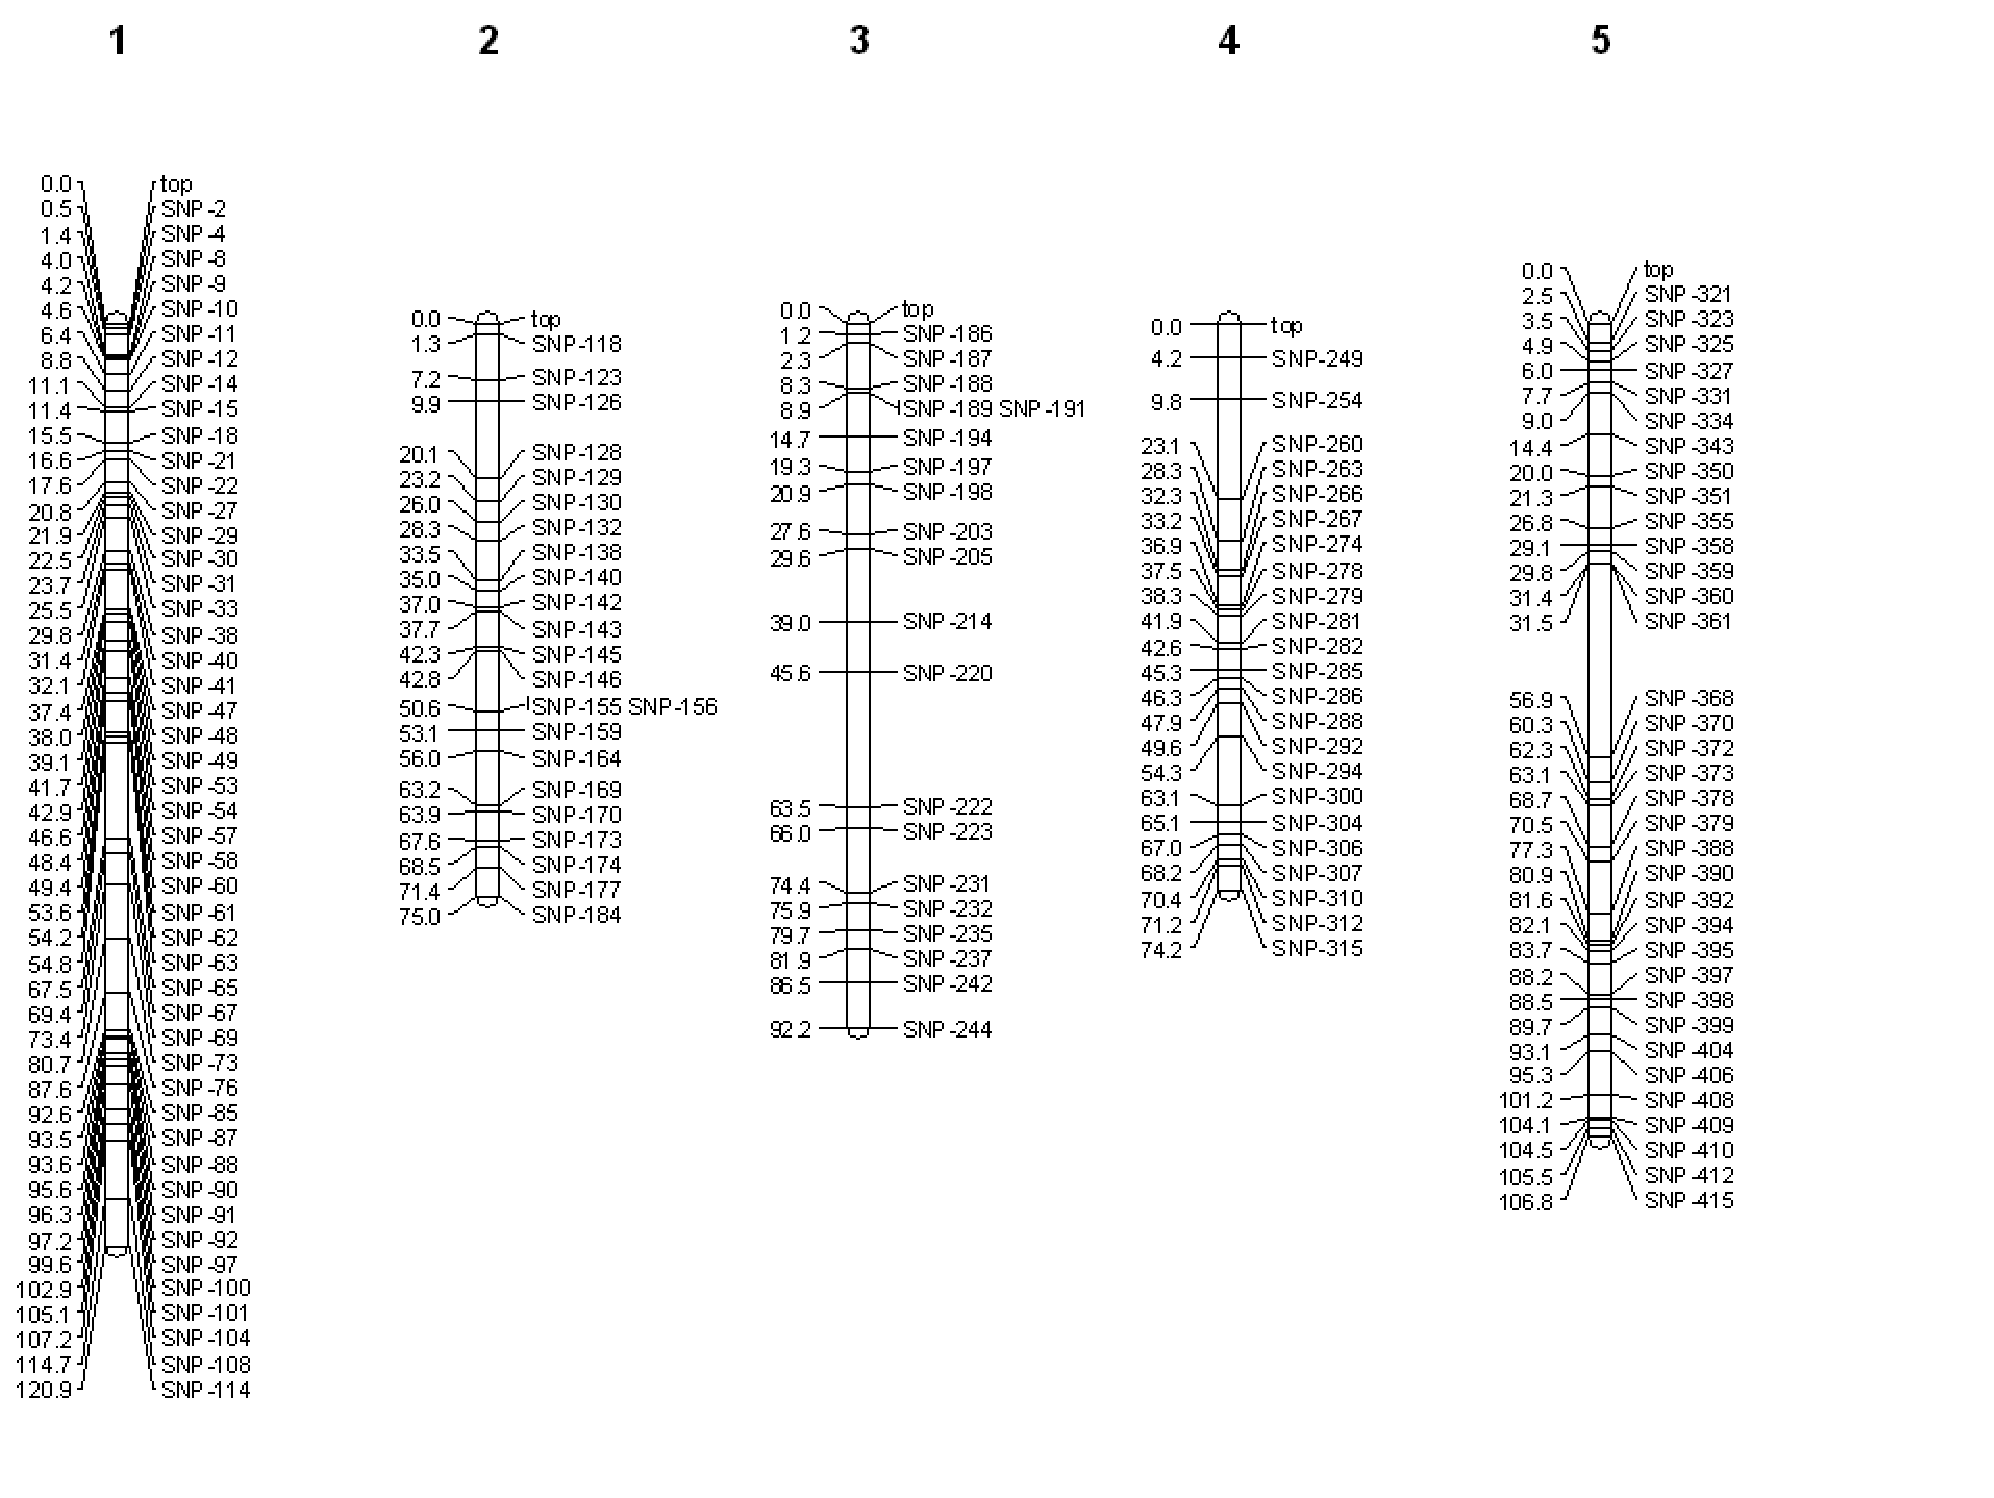
\includegraphics[width=1\textwidth]{figures/snp_locations_on_chr.eps}
\caption{}\label{f1}
\end{figure}

\section{inconsistency in duplicated calls}
The duplication arises in two situations. 1. For one strain, several runs of genotyping was carried out due to either failure of earlier experiments or lack of communication between different labs. 2. Several strains were recorded as different strains in the database.

Mentioned earlier, 640 strains with same ecotypeid has duplicated calls on one snp locus (1st kind). 89 strains out of 5679 different ecotypeid strains have same nativename and stockparent (2nd kind), which adds more to duplicated calls.

Among $(640+89)*149=108621$ genome positions, 749 (ratio=0.00689553585402) show inconsistency (more than 1 non-NA calls). A simple voting scheme is used to resolve these duplicated inconsistent call.

Final data matrix is 5590 strains by 149 snps. 10.6\% of this matrix is NA. Figure~\ref{f24} is what matrix looks like after coding different calls into integers.

\begin{figure}
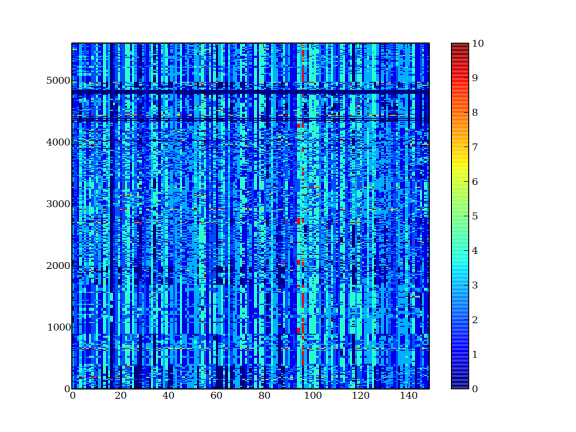
\includegraphics[width=1\textwidth]{figures/data.eps}
\caption{0 is NA. 1-4 are ACGT. 5-10 are heterozygous calls.}\label{f24}
\end{figure}

\section{Genotyping Error Rate}
The 96 strains from \cite{Nordborg2005} were genotyped again, which offered an opportunity to have a rough estimate of genotyping error rate by comparing the data from two different experiments. Figure~\ref{f0} is an overview of all the differences.

The optimistic error rate (not counting the NAs) is 121/(12408+121) = 0.96\%. Taking the NAs into account, the error rate would be (121+893+804)/( 12408.0+121+893+804) = 12.78\%.

\begin{figure}
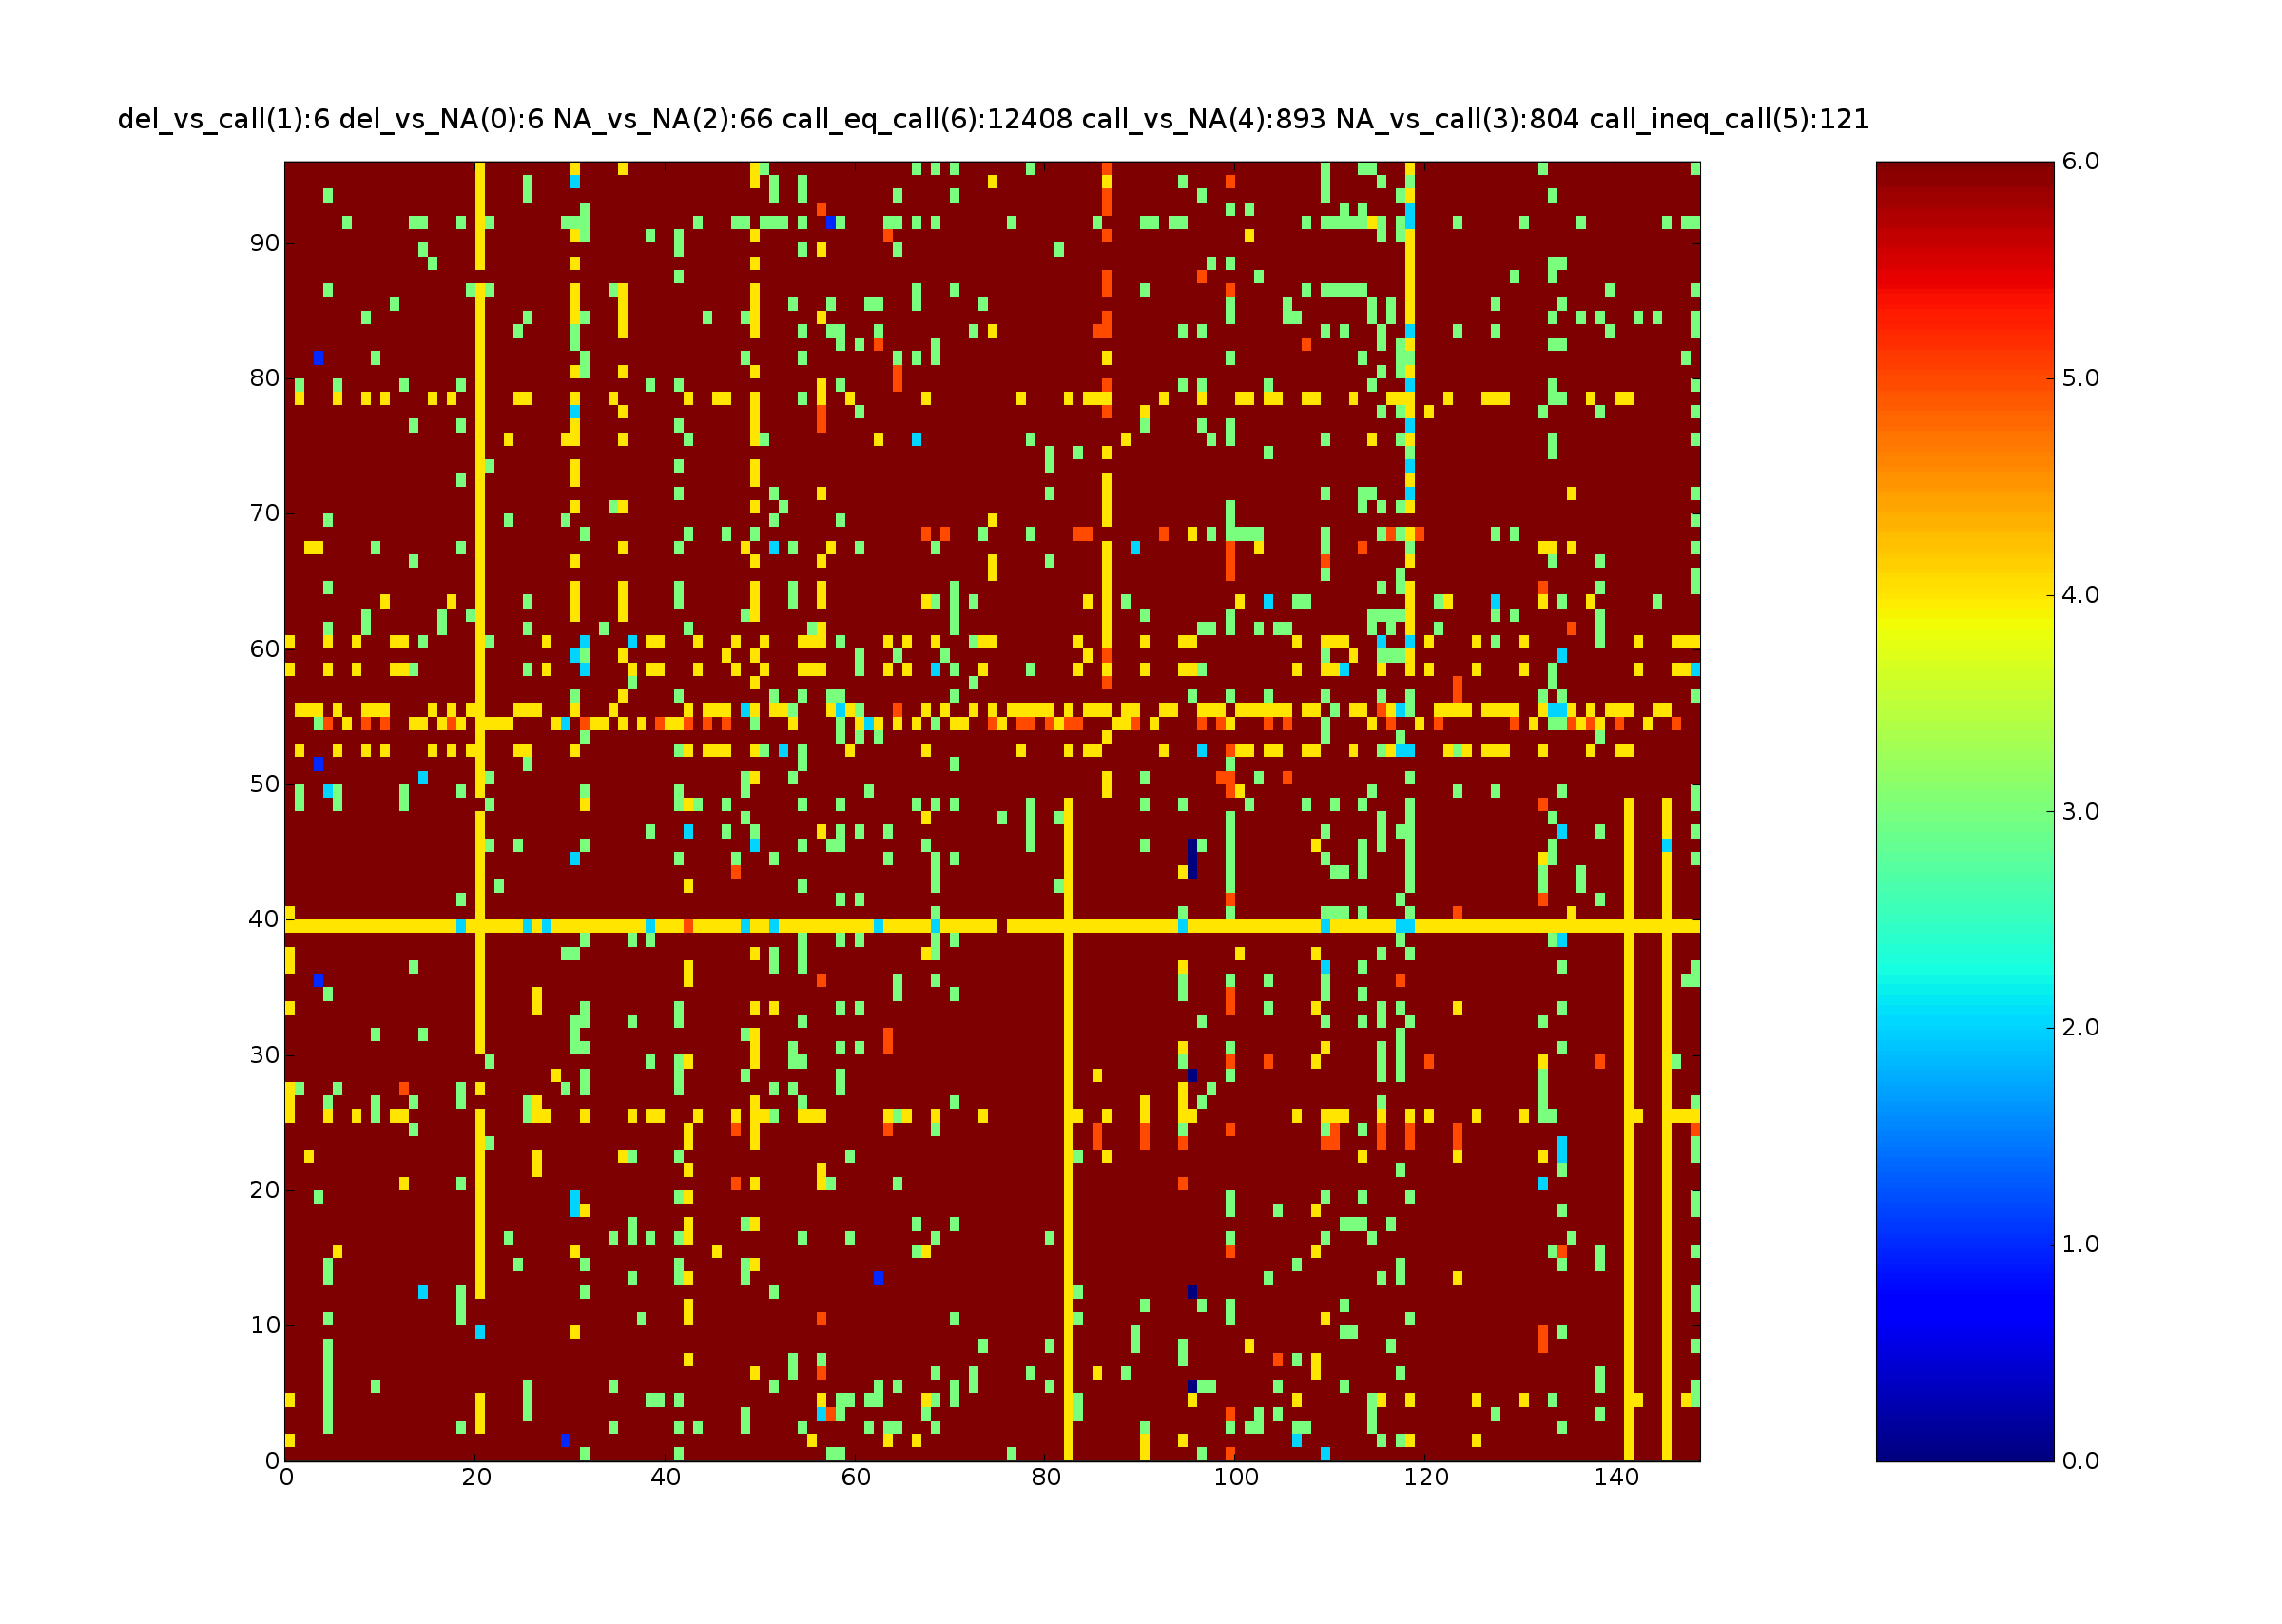
\includegraphics[width=1\textwidth]{figures/snp_matrix_2010_justin_149snps_vs_justin_data_y.eps}
\caption{2010 versus Justin}\label{f0}
\end{figure}


\section{NA Filtering}
Figure ~\ref{f10} is the Strain by SNP matrix after being sorted. A bunch of NA-rich strains are shown on top of the figure.

\begin{figure}
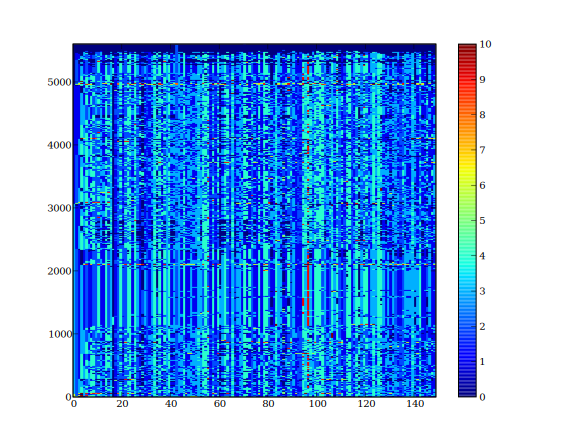
\includegraphics[width=1\textwidth]{figures/data_sorted.eps}
\caption{0 is NA. 1-4 are ACGT. 5-10 are heterozygous call}\label{f10}
\end{figure}


Figure~\ref{f4} is a histogram of NA percentage in all SNPs. 5 SNPs with $\geq 40\%$ NAs were removed. Figure~\ref{f5} is a histogram of NA percentage in all strains. 194 strains with $\geq 40\%$ NAs were removed.

\begin{figure}
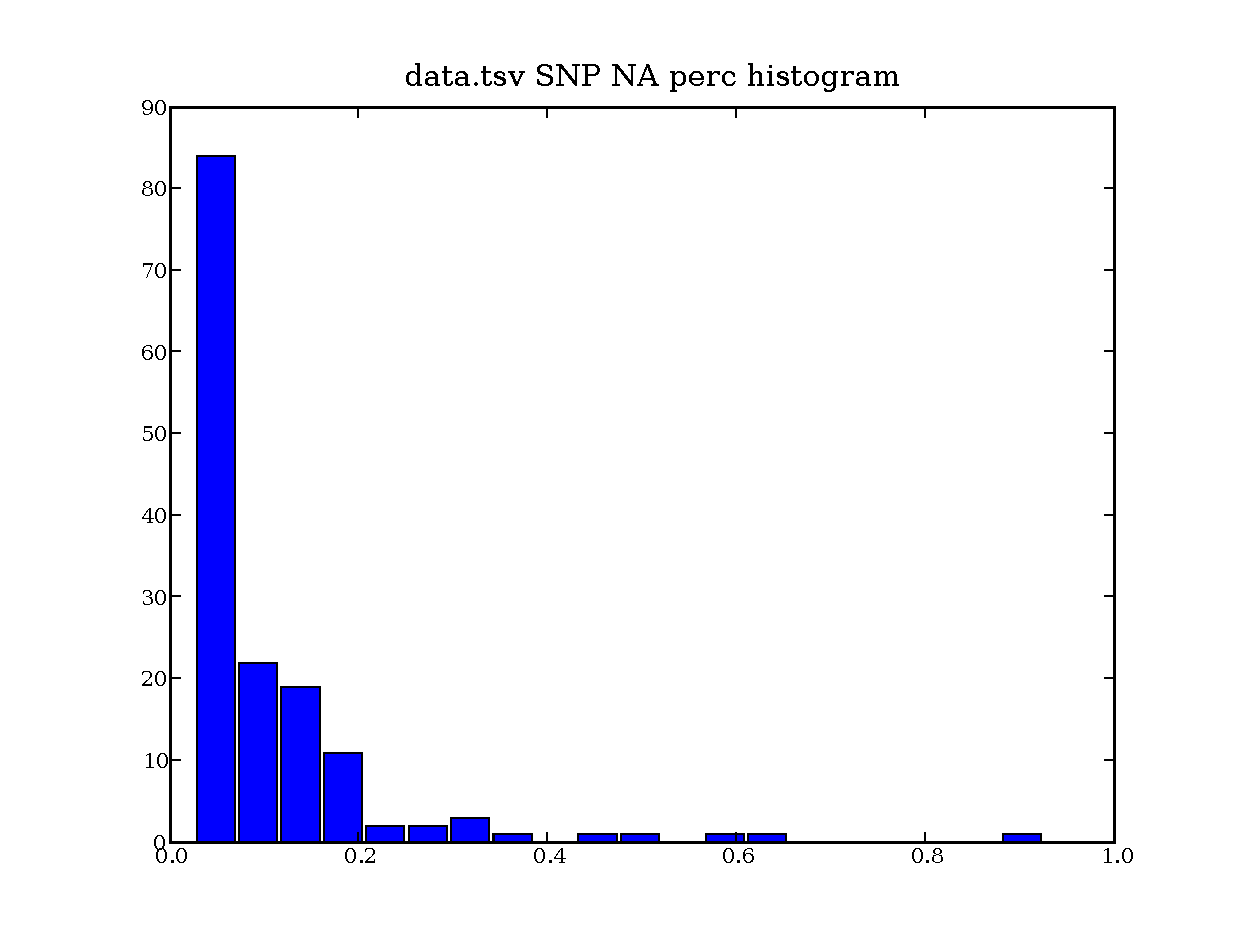
\includegraphics[width=1\textwidth]{figures/data_SNP_NA_perc.eps}
\caption{}\label{f4}
\end{figure}

\begin{figure}
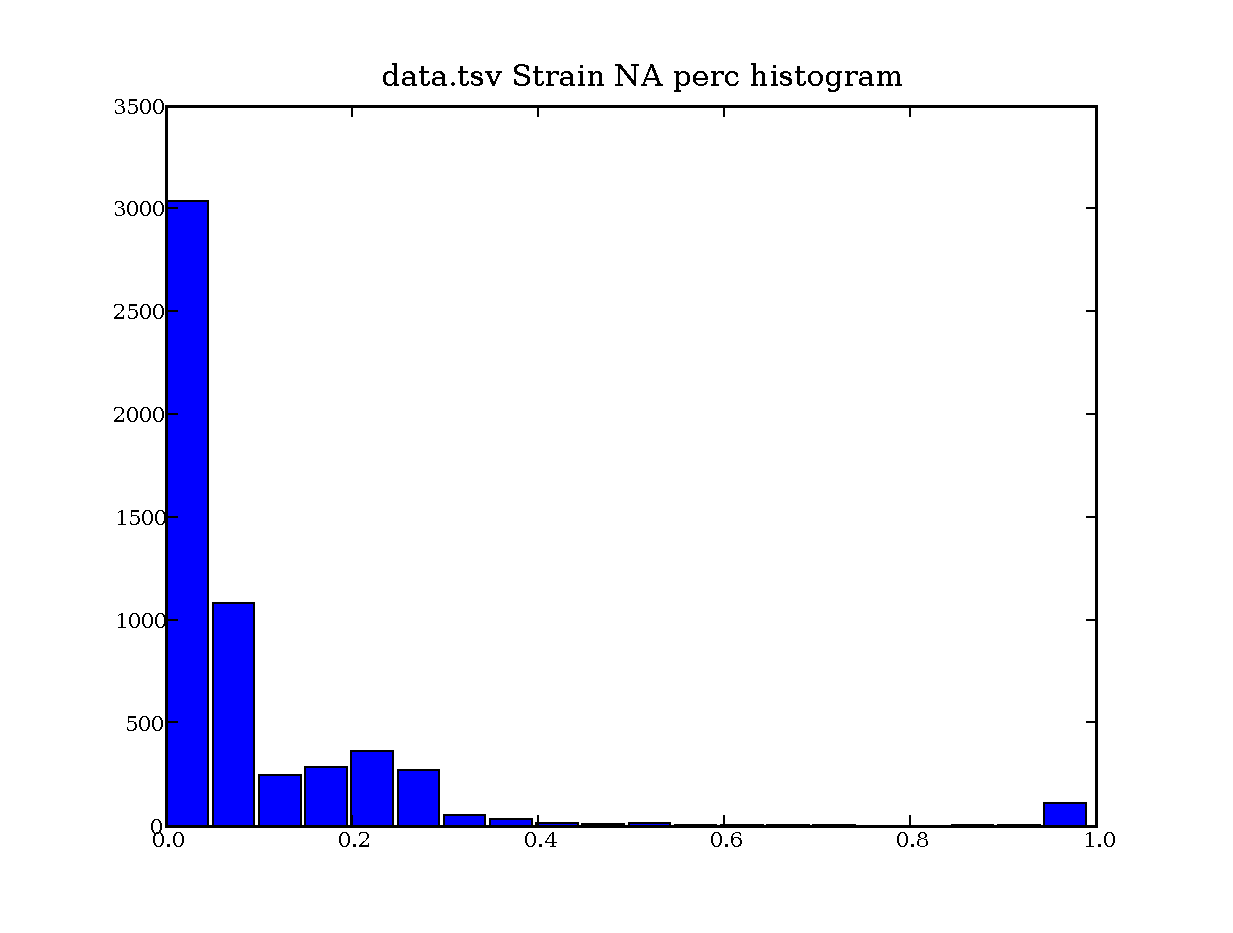
\includegraphics[width=1\textwidth]{figures/data_strain_NA_perc.eps}
\caption{}\label{f5}
\end{figure}


\section{Bogus Heterozygous Calls(column-wise)}
From figure~\ref{f24} or figure~\ref{f10}, there're columns with an unreasonable whopping number of heterozygous calls.

Check figure~\ref{f2} for the histogram of heterozygosity of each strain. Among 5590-194=5396 strains, 2407 strains have no heterozygous calls. 1961 strains have only one heterozygous call. None of the strains' heterozygosity exceeds 0.5.

\begin{figure}
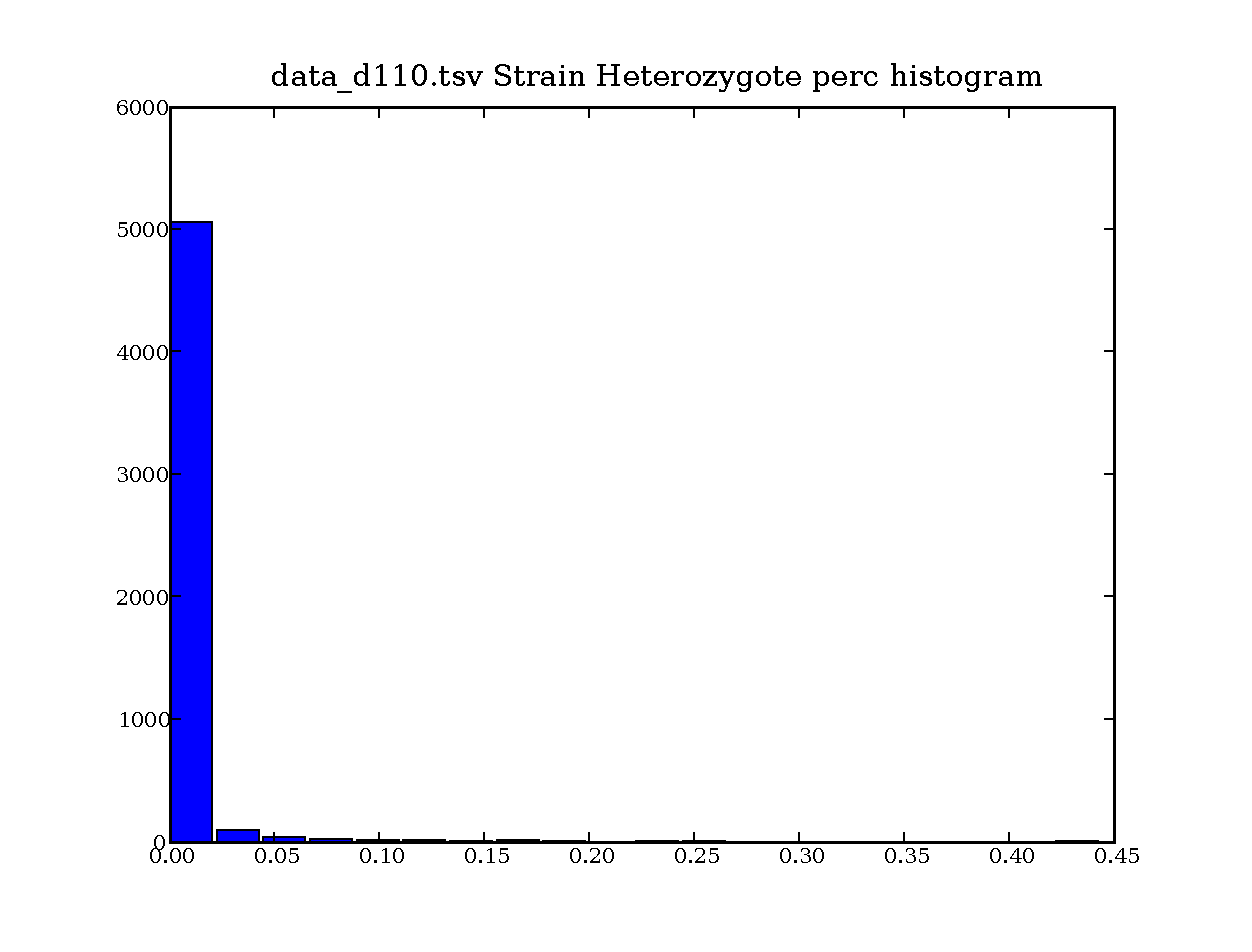
\includegraphics[width=1\textwidth]{figures/data_d110_strain_hz_perc.eps}
\caption{}\label{f2}
\end{figure}

A simple statistical model is used to quantitively tell how unreasonable each column is.

\subsection{model for snp locus}
\begin{equation}
P({SNP}_j|Strain\quad heterozygous\quad info) = \prod_{i=1}^{N} p_i^{a_i^j} (1-p_i)^{1-a_i^j}
\end{equation}

$p_i$ is probability that one strain has heterozygous call.

$a_i^j$ is indicator whether ${SNP}_j$ is homozygous($=1$) or not($=0$) for ${Strain}_i$.

Figure~\ref{f3} is the histogram of the probability for each SNP locus after taking logarithm.

\begin{figure}
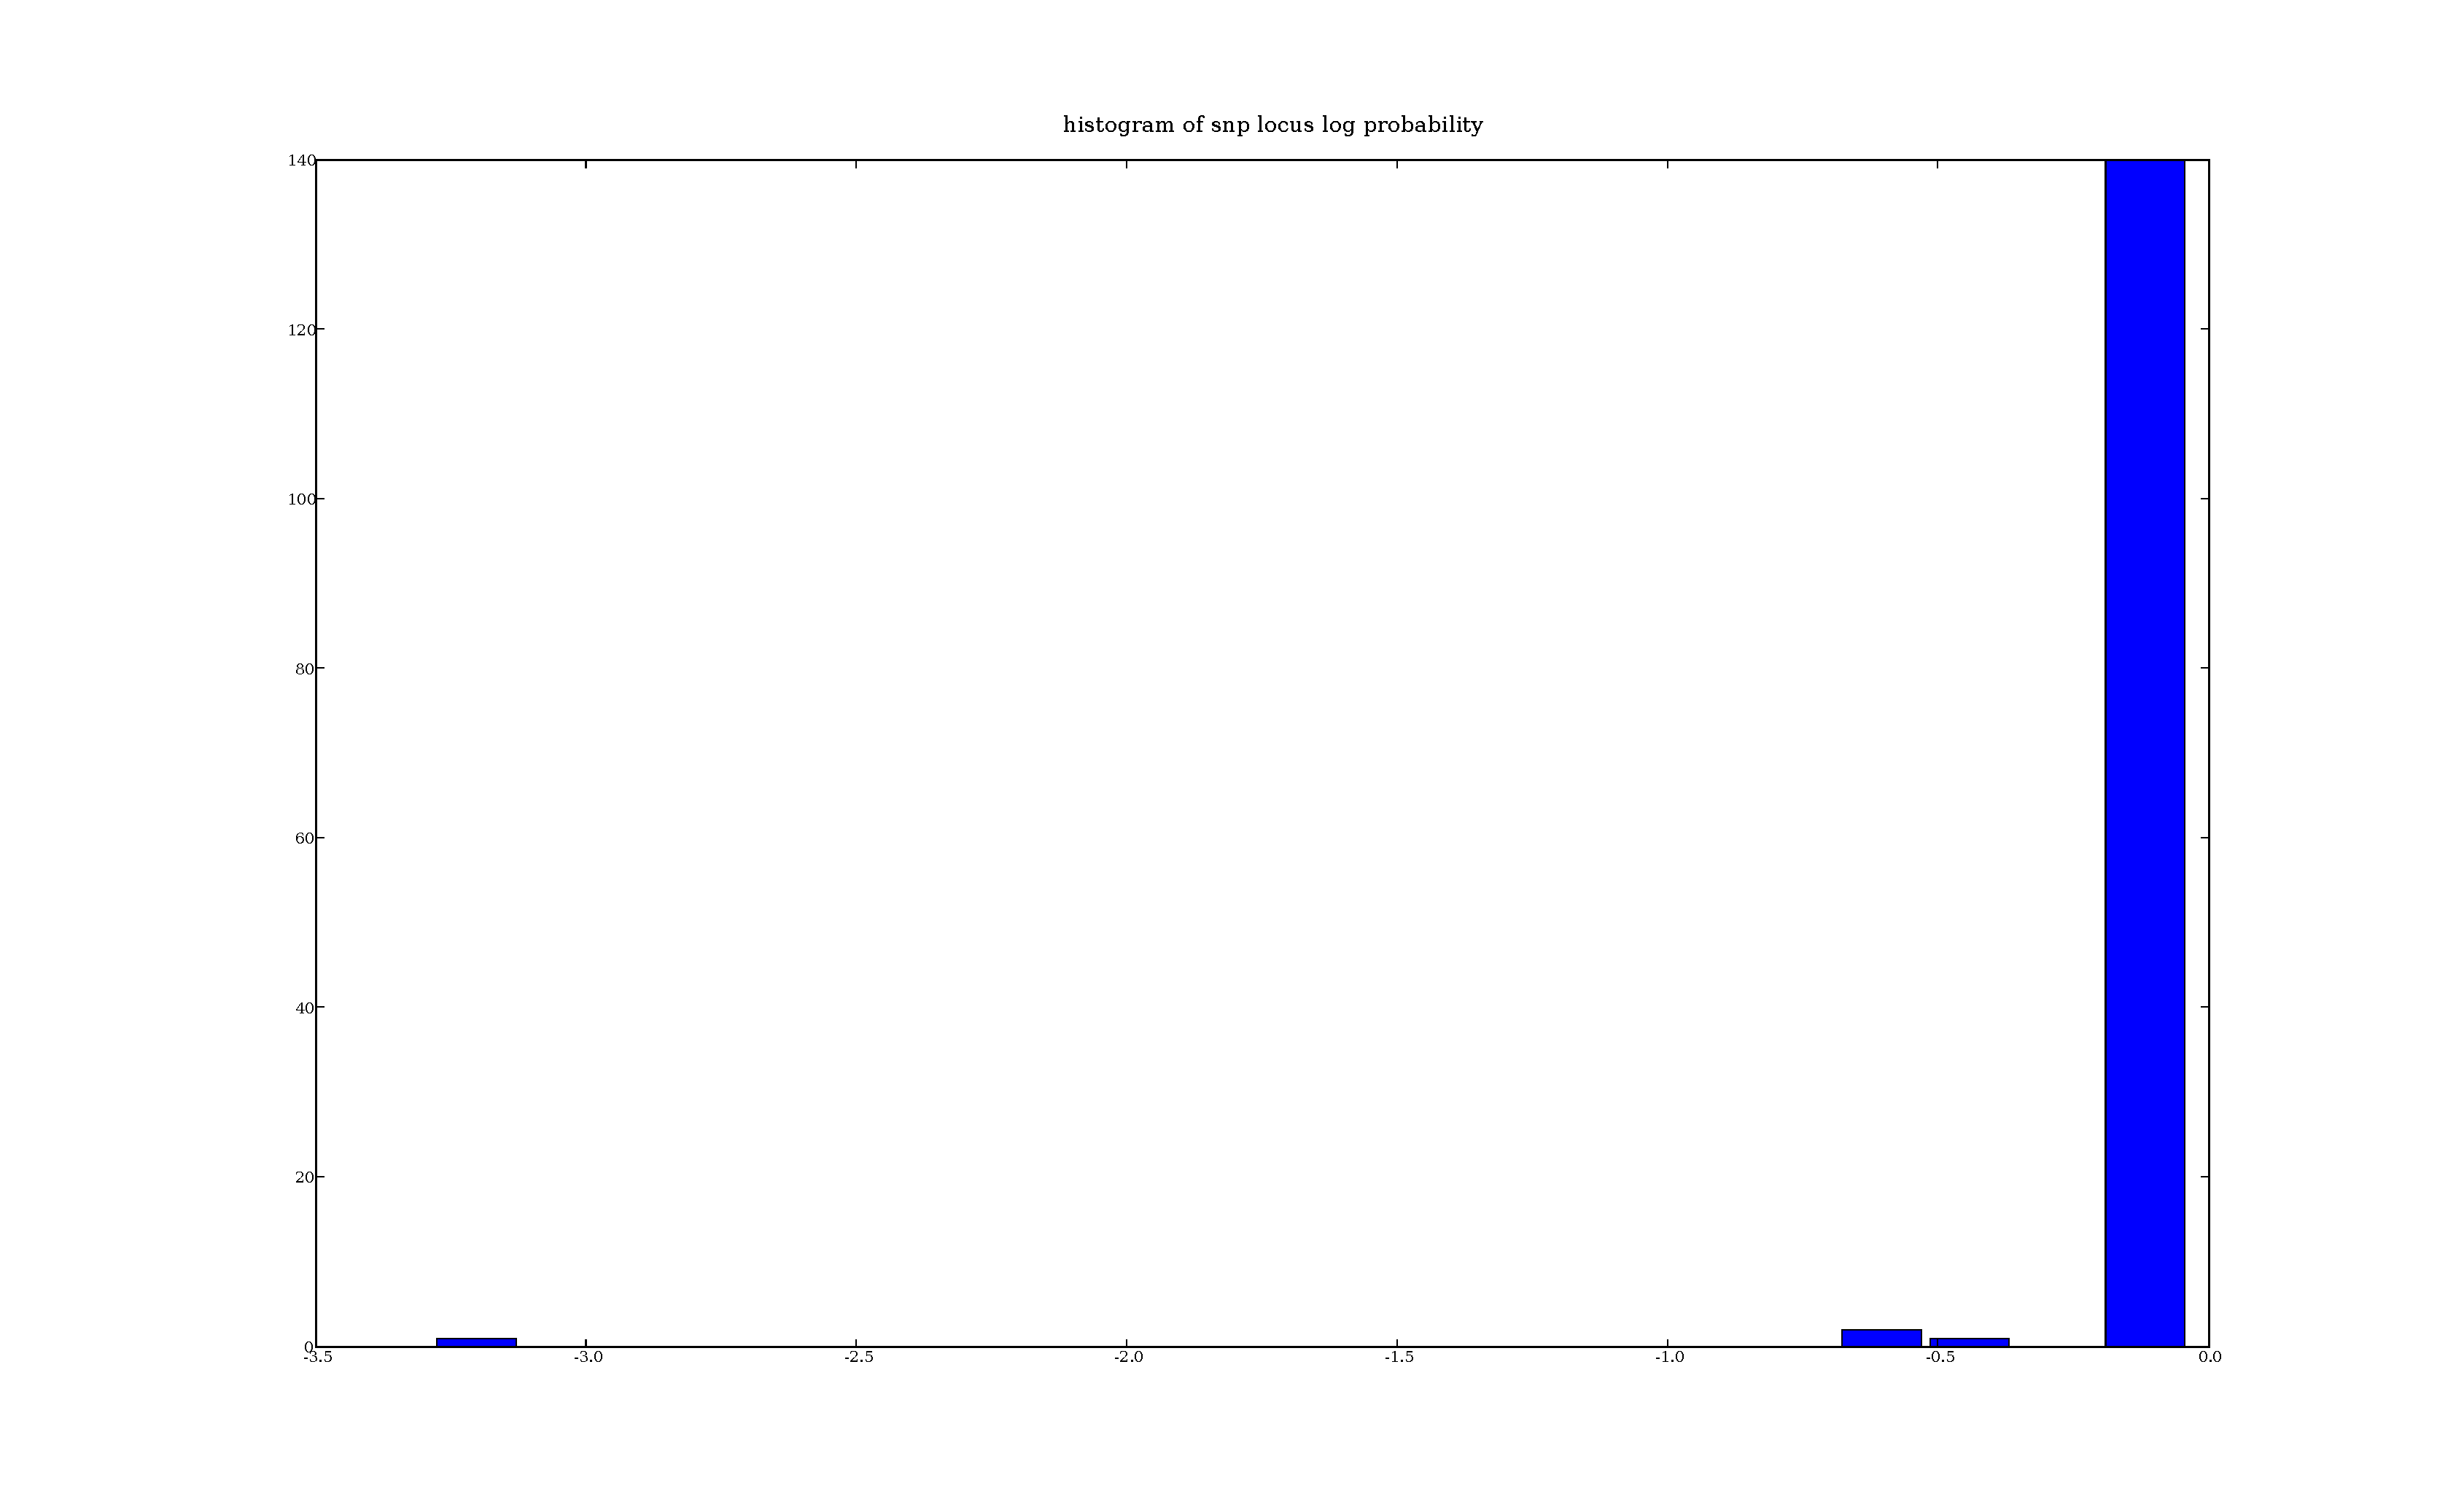
\includegraphics[width=1\textwidth]{figures/data_d110_c0_5_SNP_locus_log_prob.eps}
\caption{}\label{f3}
\end{figure}

4 SNP loci with log probability $\leq -0.5$ were removed. These four loci show long stretch of heterozygous calls among lots of strains in Figure~\ref{f2}. 

These long stretch of heterozygous calls could trace to technical error, segmental duplication in all strains, segmental duplication in some strains  or real heterozygotes caused by population structure.


\section{identity strains across globe}
Here is to see how identity strain pairs are distributed across globe. We first tried a loose criteria to define identity. If one of the two calls is NA, it's deemed as identical too. Hence, the transivity of identity relationship is not guaranteed. For example, given strain 1 and 2 are identical and strain 1 and 3 are also identical, strain 1 and 3 might not be identical.

In total, there're 433,295 identity pairs. Think of it as a graph, which can be partitioned into connected components. Within each connected component, any two strains could be reached via some intermediate strains based on identity relationship. Each connected component could loosely correspond to a distinct haplotype ('loosely' because its transivity is not guaranteed and there're still some strains who are not identical.).

\subsection{connected components in the identity strain graph}
There're not many long-distance connected components. Most of them are within one country. So far two components were spotted as cross ocean.(still need systematically determine how many cross-ocean components there are.)

Figure~\ref{f25} shows the cross-atlantic component. Figure~\ref{f26} is the data matrix corresponding to the cross-atlantic component. Notice this component is actually a clique (transivity reached, any two strains are identical to each other.). Magnus and I just sat down and found three Col-0 strains are in this component, which raises lab-contamination suspicion over this component. This component is probably Col-0 haplotype.

There's another component linking america and japan, figure~\ref{f27}. the picture was cut improperly. Check figure~\ref{f22} to see it's actually connected all the way to japan.

\begin{figure}
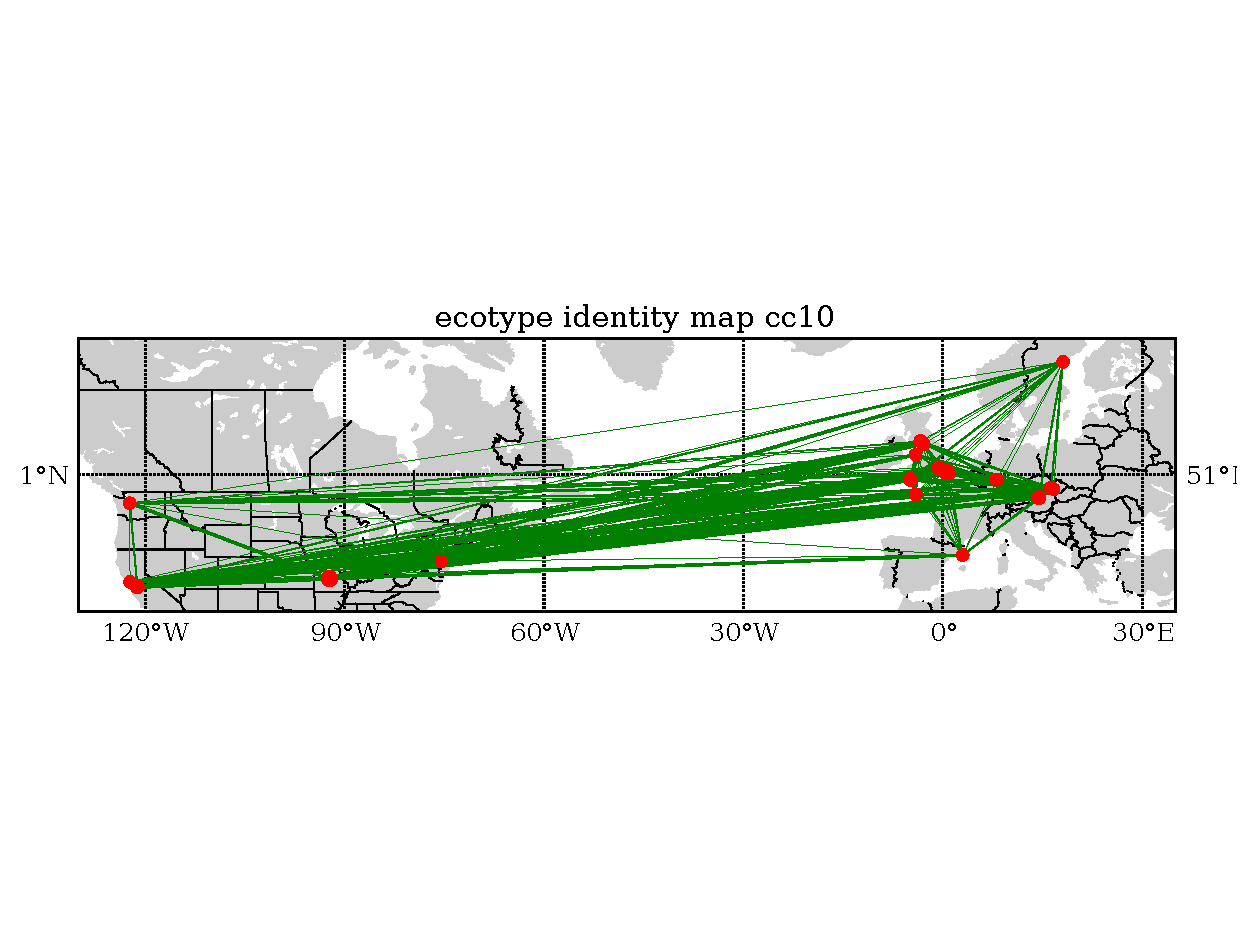
\includegraphics[width=1\textwidth]{figures/ecotype_identity_cc10_site_network.eps}
\caption{the cross-atlantic component}\label{f25}
\end{figure}

\begin{figure}
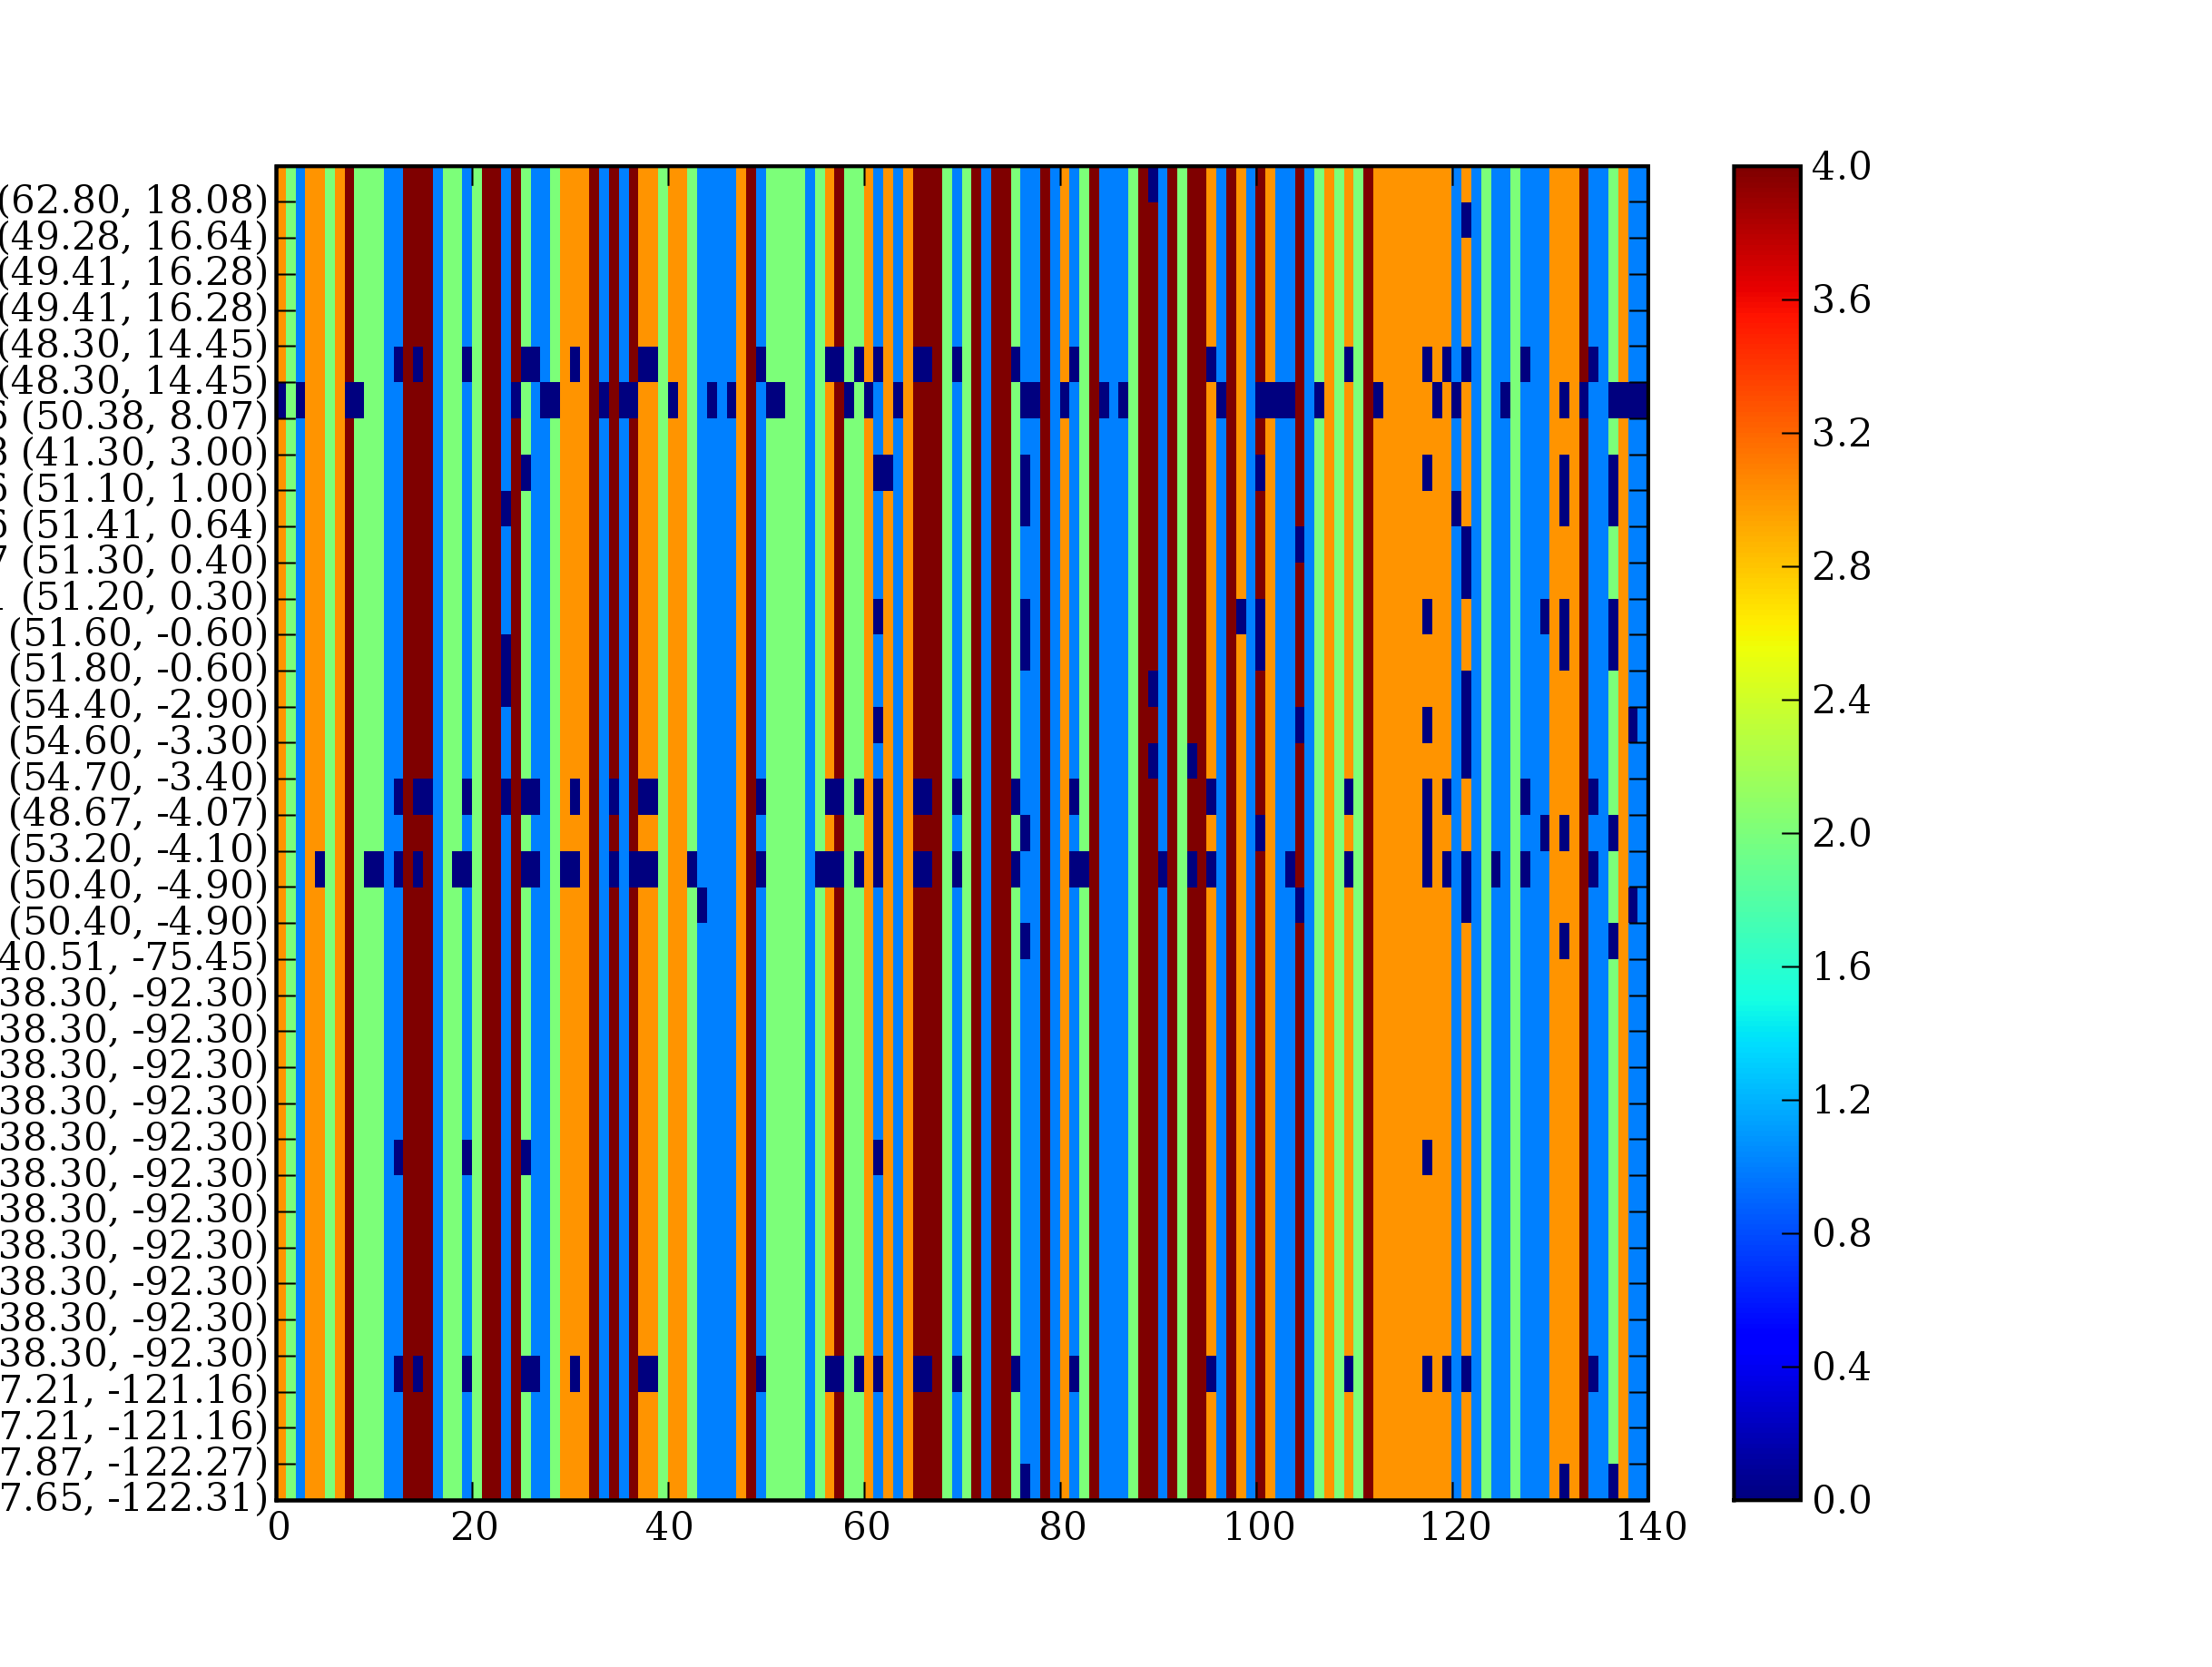
\includegraphics[width=1\textwidth]{figures/ecotype_identity_map_cc10.eps}
\caption{the data corresponding to the cross-atlantic component in figure~\ref{f25}}\label{f26}
\end{figure}

\begin{figure}
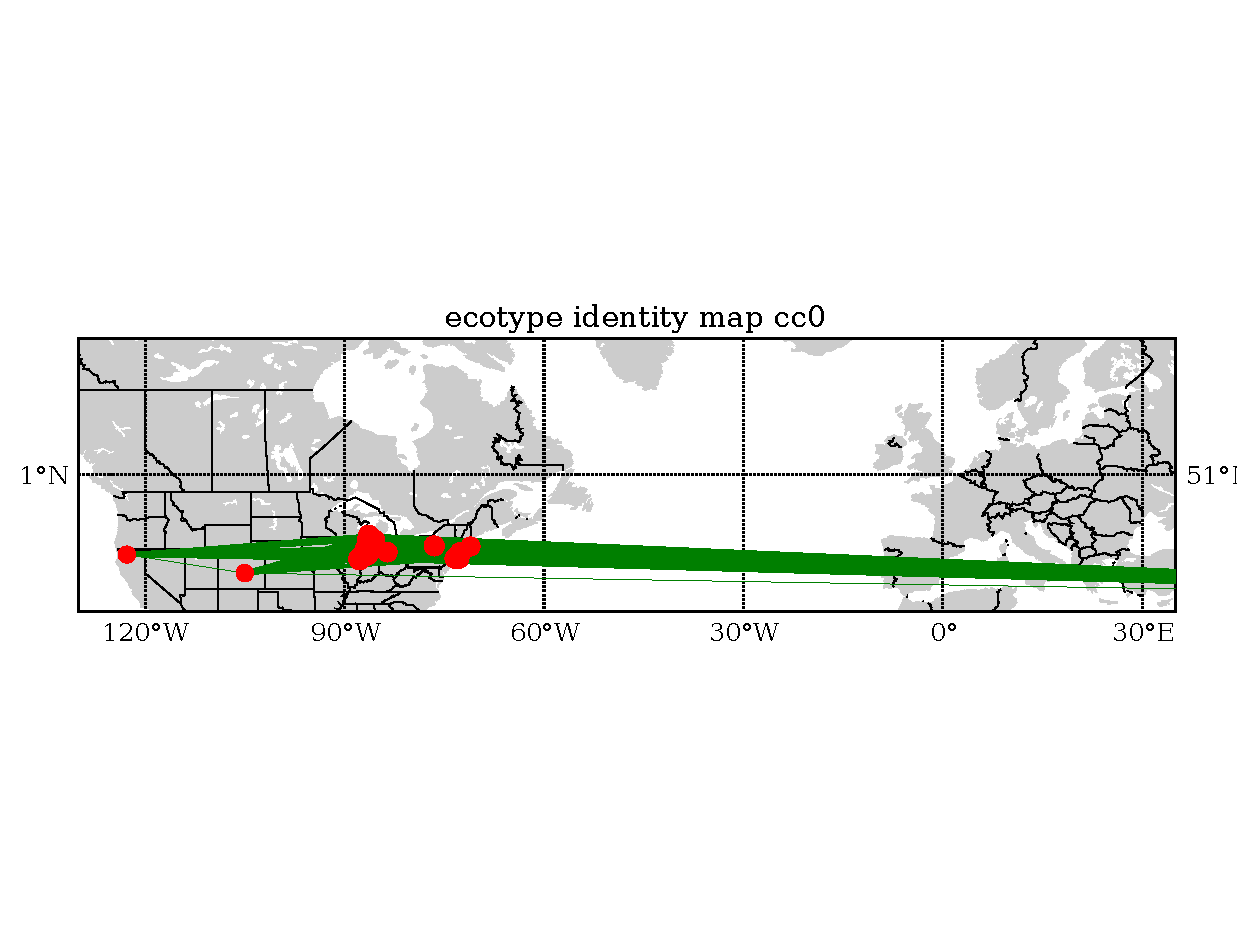
\includegraphics[width=1\textwidth]{figures/ecotype_identity_cc0_site_network.eps}
\caption{the america-japan component}\label{f27}
\end{figure}

\subsection{Identity Map on the scale of population}
In order to gain a global look. we grouped strains into population. Each population is formed via connecting close sites. There's a distance (great circle distance) threshold to determine how close sites within a population should be.

289,867(66.9\%) pairs are across-population for population model thresholded by 25km. In figure~\ref{f22}, Each population is denoted as a red dot with its diameter proportional to the number of identity pairs within that population. An edge is connected if there's identity relationship between two populations. The thickness of an edge corresponds to the number identity pairs between them.

\begin{figure}
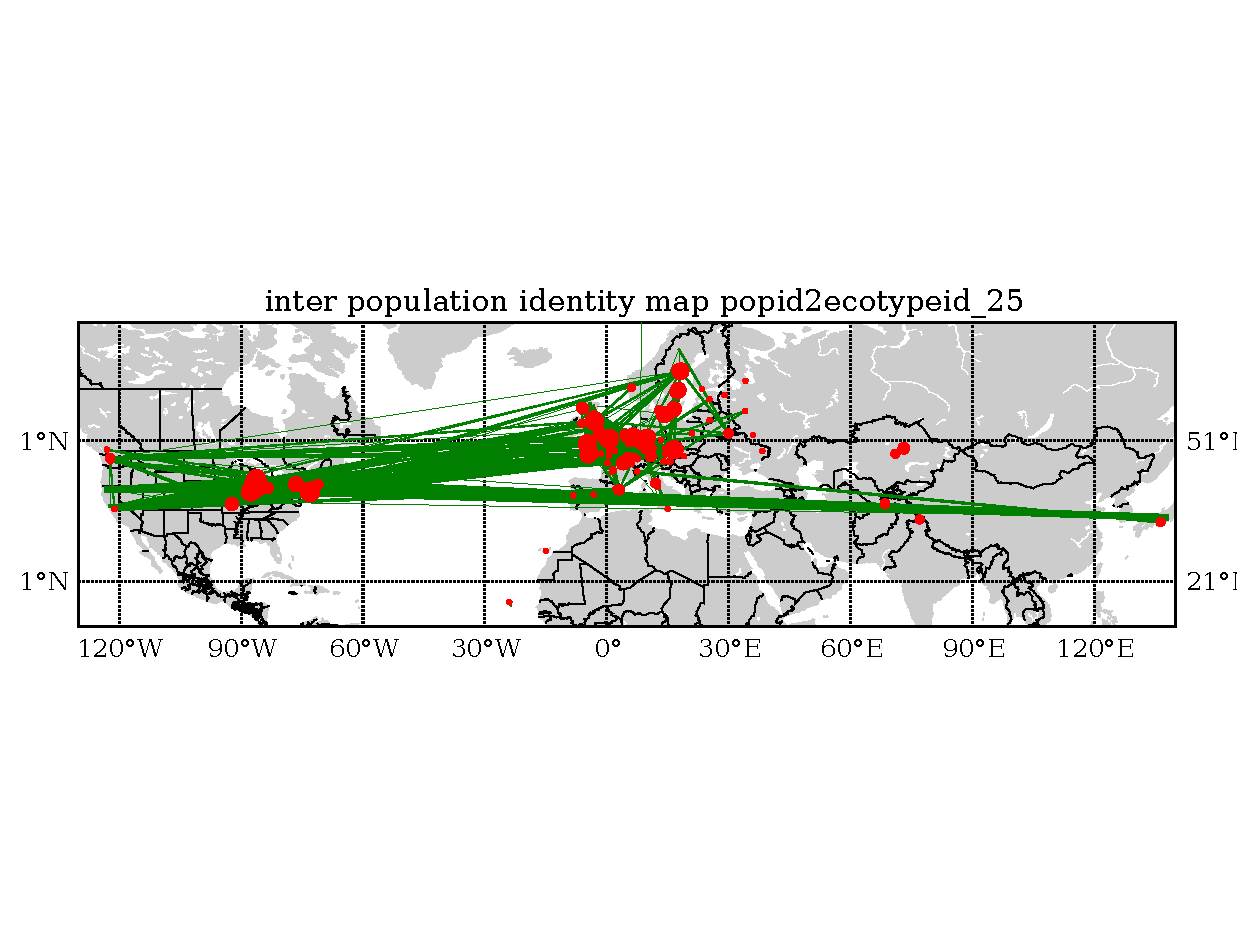
\includegraphics[width=1\textwidth]{figures/identity_map1_site_network.eps}
\caption{Population Identity Map}\label{f22}
\end{figure}


\subsection{thinning the identity pairs by removing ambiguous NA-rich strains}
To enable component to reach transivity (true haplotype), magnus suggested a thinning algorithm.

Sort the individuals so that those with the smallest numbers of NA come on top.  Go through the individuals one at a time: if an individual is different (has a mismatch, ignoring NA) from one you have seen, add it to the list of unique haplotypes.

Given the list of unique haplotypes. Now go through the remainder and assign those that can be assigned uniquely (no mismatches).  Leave the ones that cannot be assigned uniquely unassigned.

this is a greedy algorithm, which can't gaurantee the transivity. (another algorithm is on the way to settle this...)

the number of identity pairs dropped to 364801 (15\% less) but the inter population identities percentage, 244826/364801=0.67112206381 is almost same as before.

Figure~\ref{f28} is the identity map after thinning. global pattern is still there. and two cross-ocean components are still there (data not shown).

\begin{figure}
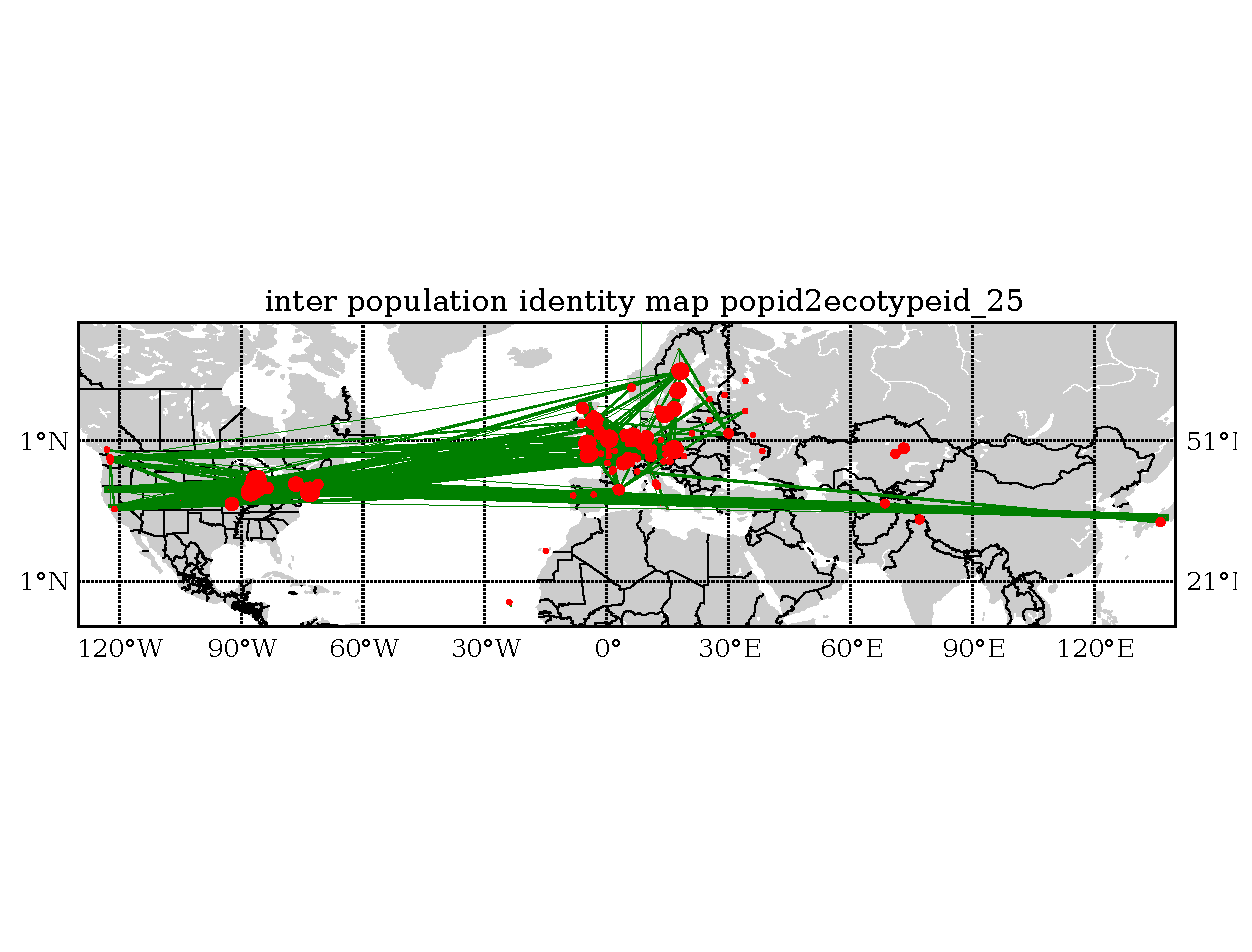
\includegraphics[width=1\textwidth]{figures/identity_map2_complete_site_network.eps}
\caption{Population Identity Map after thinning}\label{f28}
\end{figure}

\section{Remove Identity Strains}
Due to the highly inbreeding nature of Arabidopsis, there're lots of identity strains in the samples collected from nature. In Figure~\ref{f10}, blocks of identity strains are very obvious. In the detection of identity strains, NA is regarded to be identical to any genotyping call. Because different strains have NAs in different SNP loci, the identity relation is not transitive. For example, A is identical to B and B is identical to C but A might not be identical to C. A graph is constructed with strains as nodes and two nodes are connected if these two strains are deemed as identical. An example graph is shown in Figure ~(?). A greedy algorithm is used to remove nodes with highest degree until no edges left.

In the end, 2575 strains were removed.

\section{Detecting Recombinant Inbred Line(RIL)}
Figure~\ref{f6} is a diagram showing the production of recombinant imbred lines by selfing.

use Dynamic programming to identify RILs with minimum number of recombinations. Regardless of how many selfing generations, the algorithm tells you whether one strain results from the outcrossing of two strains.

This step gives out results flooded with false trios. The 1st kind of false trio is that one parent is very close to the child, the other is a little farther (but still with substantial similarity) and just help to save some few incompatibilites. The 2nd kind is that one parent and child are close. The other parent is kind of irrelevant and saves the incompatibilites by being 'NA'.

\section{Estimate the number of selfing generations since the last outcrossing event}
Figure~\ref{f6} is a diagram showing the production of recombinant imbred lines by selfing. F1 would be 0 selfing generation away from the last outcrossing event as it's the direct result of outcrossing. F2 is 1 selfing generation away from the last outcrossing event.

\begin{figure}
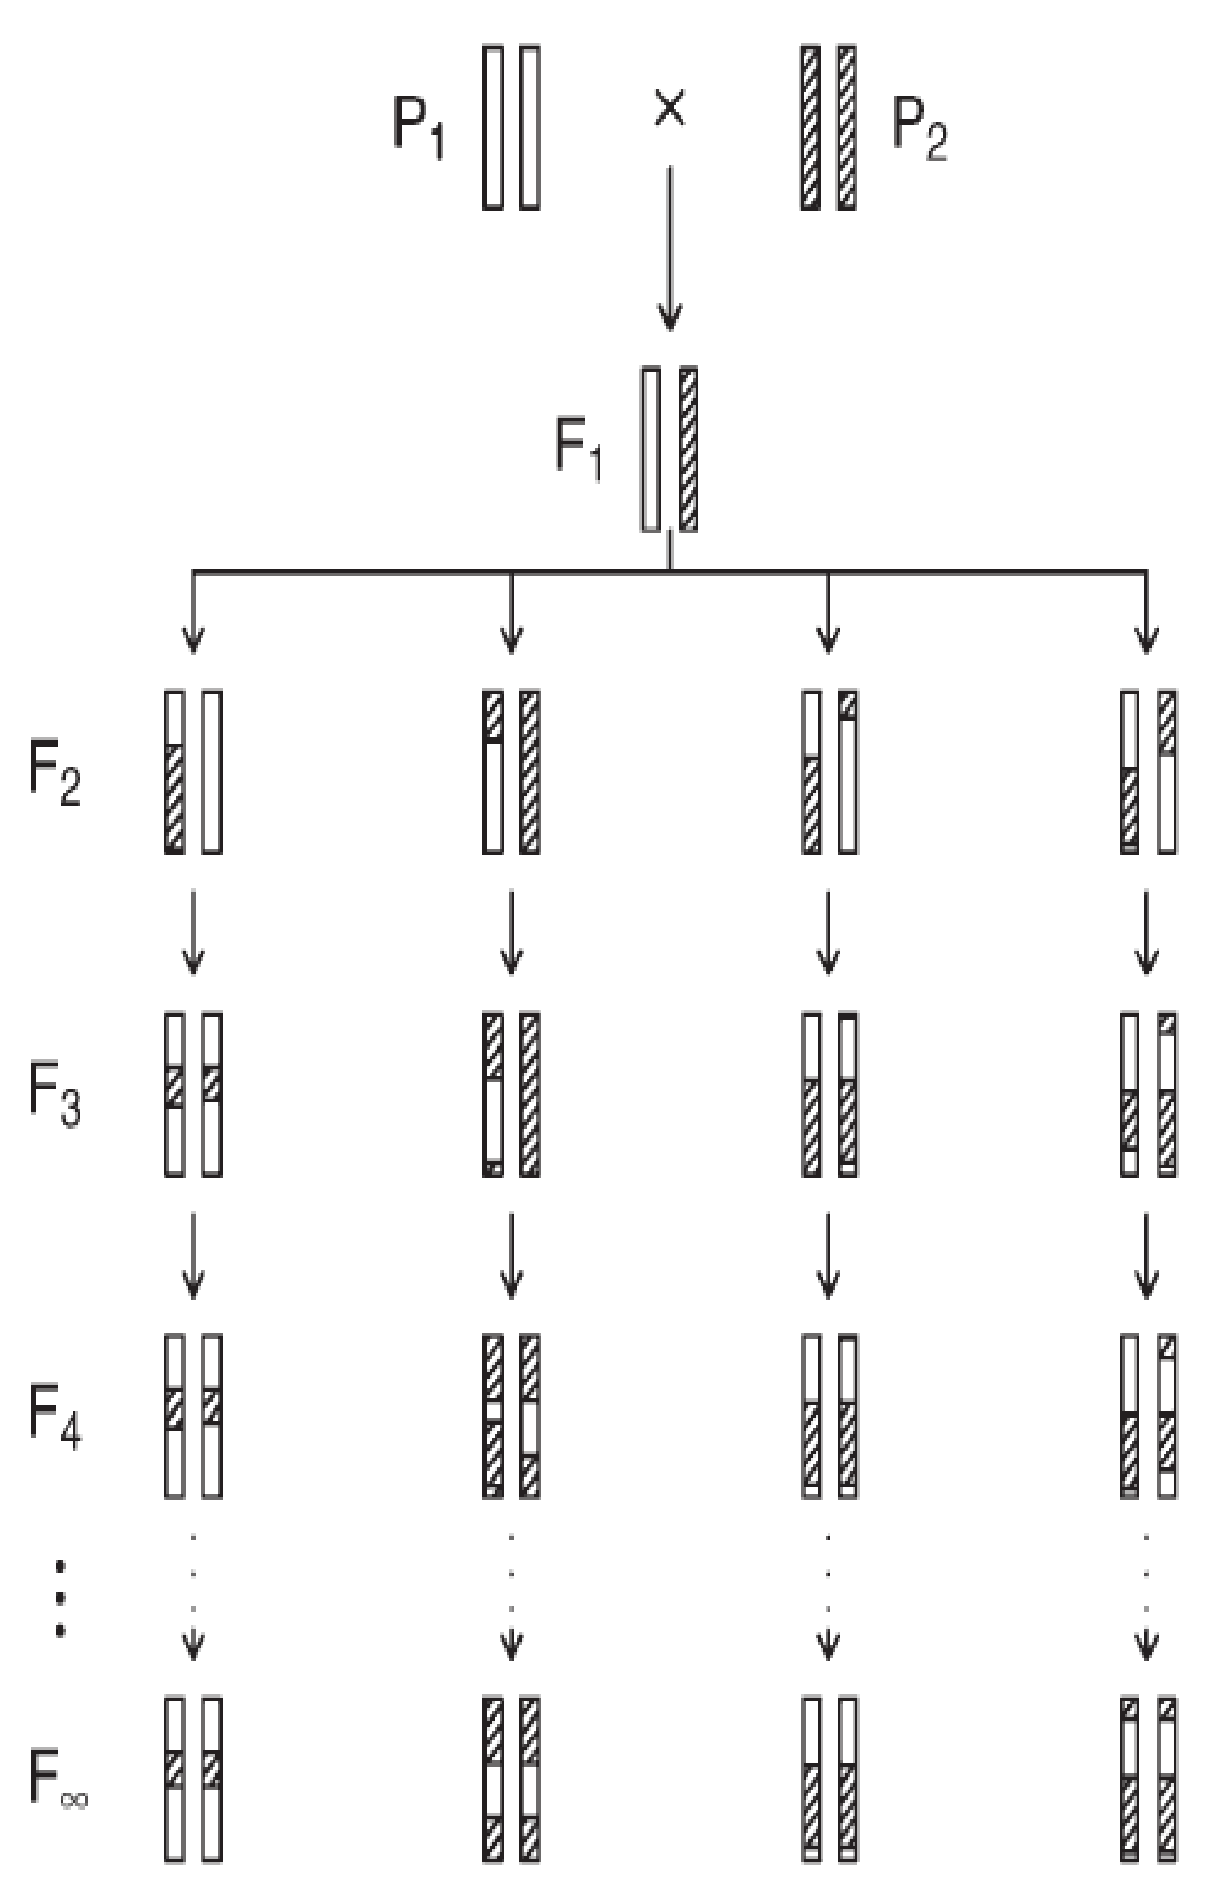
\includegraphics[width=1\textwidth]{figures/selfing_diagram.eps}
\caption{from \cite{Broman2005}}\label{f6}
\end{figure}

The following model is from \cite{Enjalbert2000}.

\subsection{model to estimate the number of selfing generations since the last outcrossing event}
\begin{equation}
D_i = 1 - \sum_{j=1}^k p_{ij}^2
\end{equation}


$p_{ij}$ is probability of allele j of SNP i. k is the number of alleles.

$D_i$ is probability of SNP i being heterozygous.


\begin{equation}
likelihood(S_n) = \prod_{i=1}^L {(\frac{D_i}{2^n})}^{a_i} {(1-\frac{D_i}{2^n})}^{1-a_i}
\end{equation}

$S_n$ is the strain which is n selfing generations away from the last outcrossing event.

$L$ is the number of loci.

$a_i$ is indicator whether SNP i is heterozygous($=1$) or not($=0$).

$\hat{n}$ is the MLE.

This model assumes the independence among the SNP loci, which is not true in general due to LD. According the recent Kim et al.(2007) paper (in preparation), LD decays within 10kb on average. In our data, the spacing between neighboring SNP loci is generally huge (see Figure~\ref{f7}). If sorted, the list of gaps between loci looks like 1713, 4520, 13250, 49053, ..., 4482219, 6334701. So only the first two gaps are within 10kb frame. So statistical independence could be well assumed.

\begin{figure}
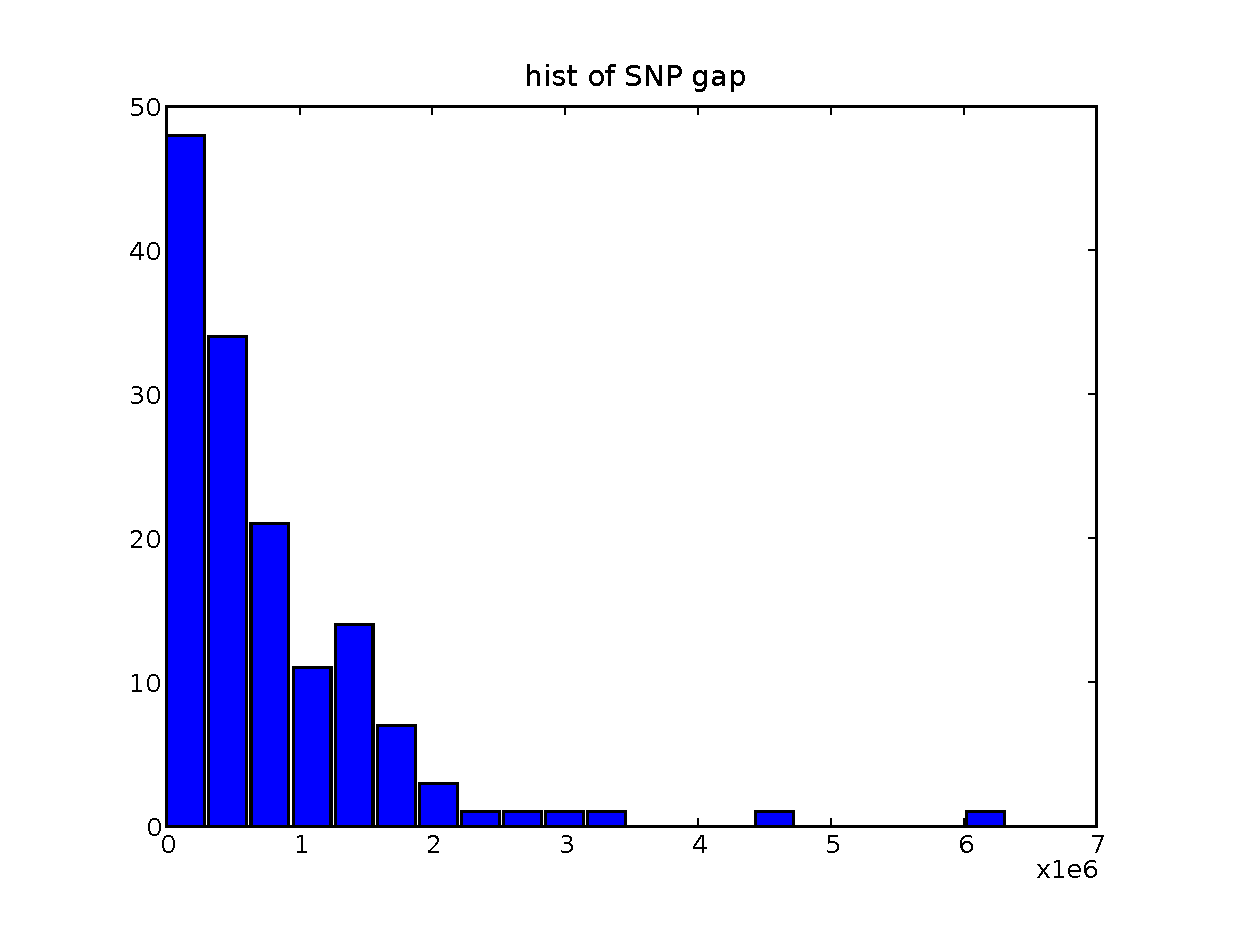
\includegraphics[width=1\textwidth]{figures/snp_locus_gap_hist.eps}
\caption{}\label{f7}
\end{figure}

Figure~\ref{f8} is the result. The spike in 6 is probably spurious estimates.

\begin{figure}
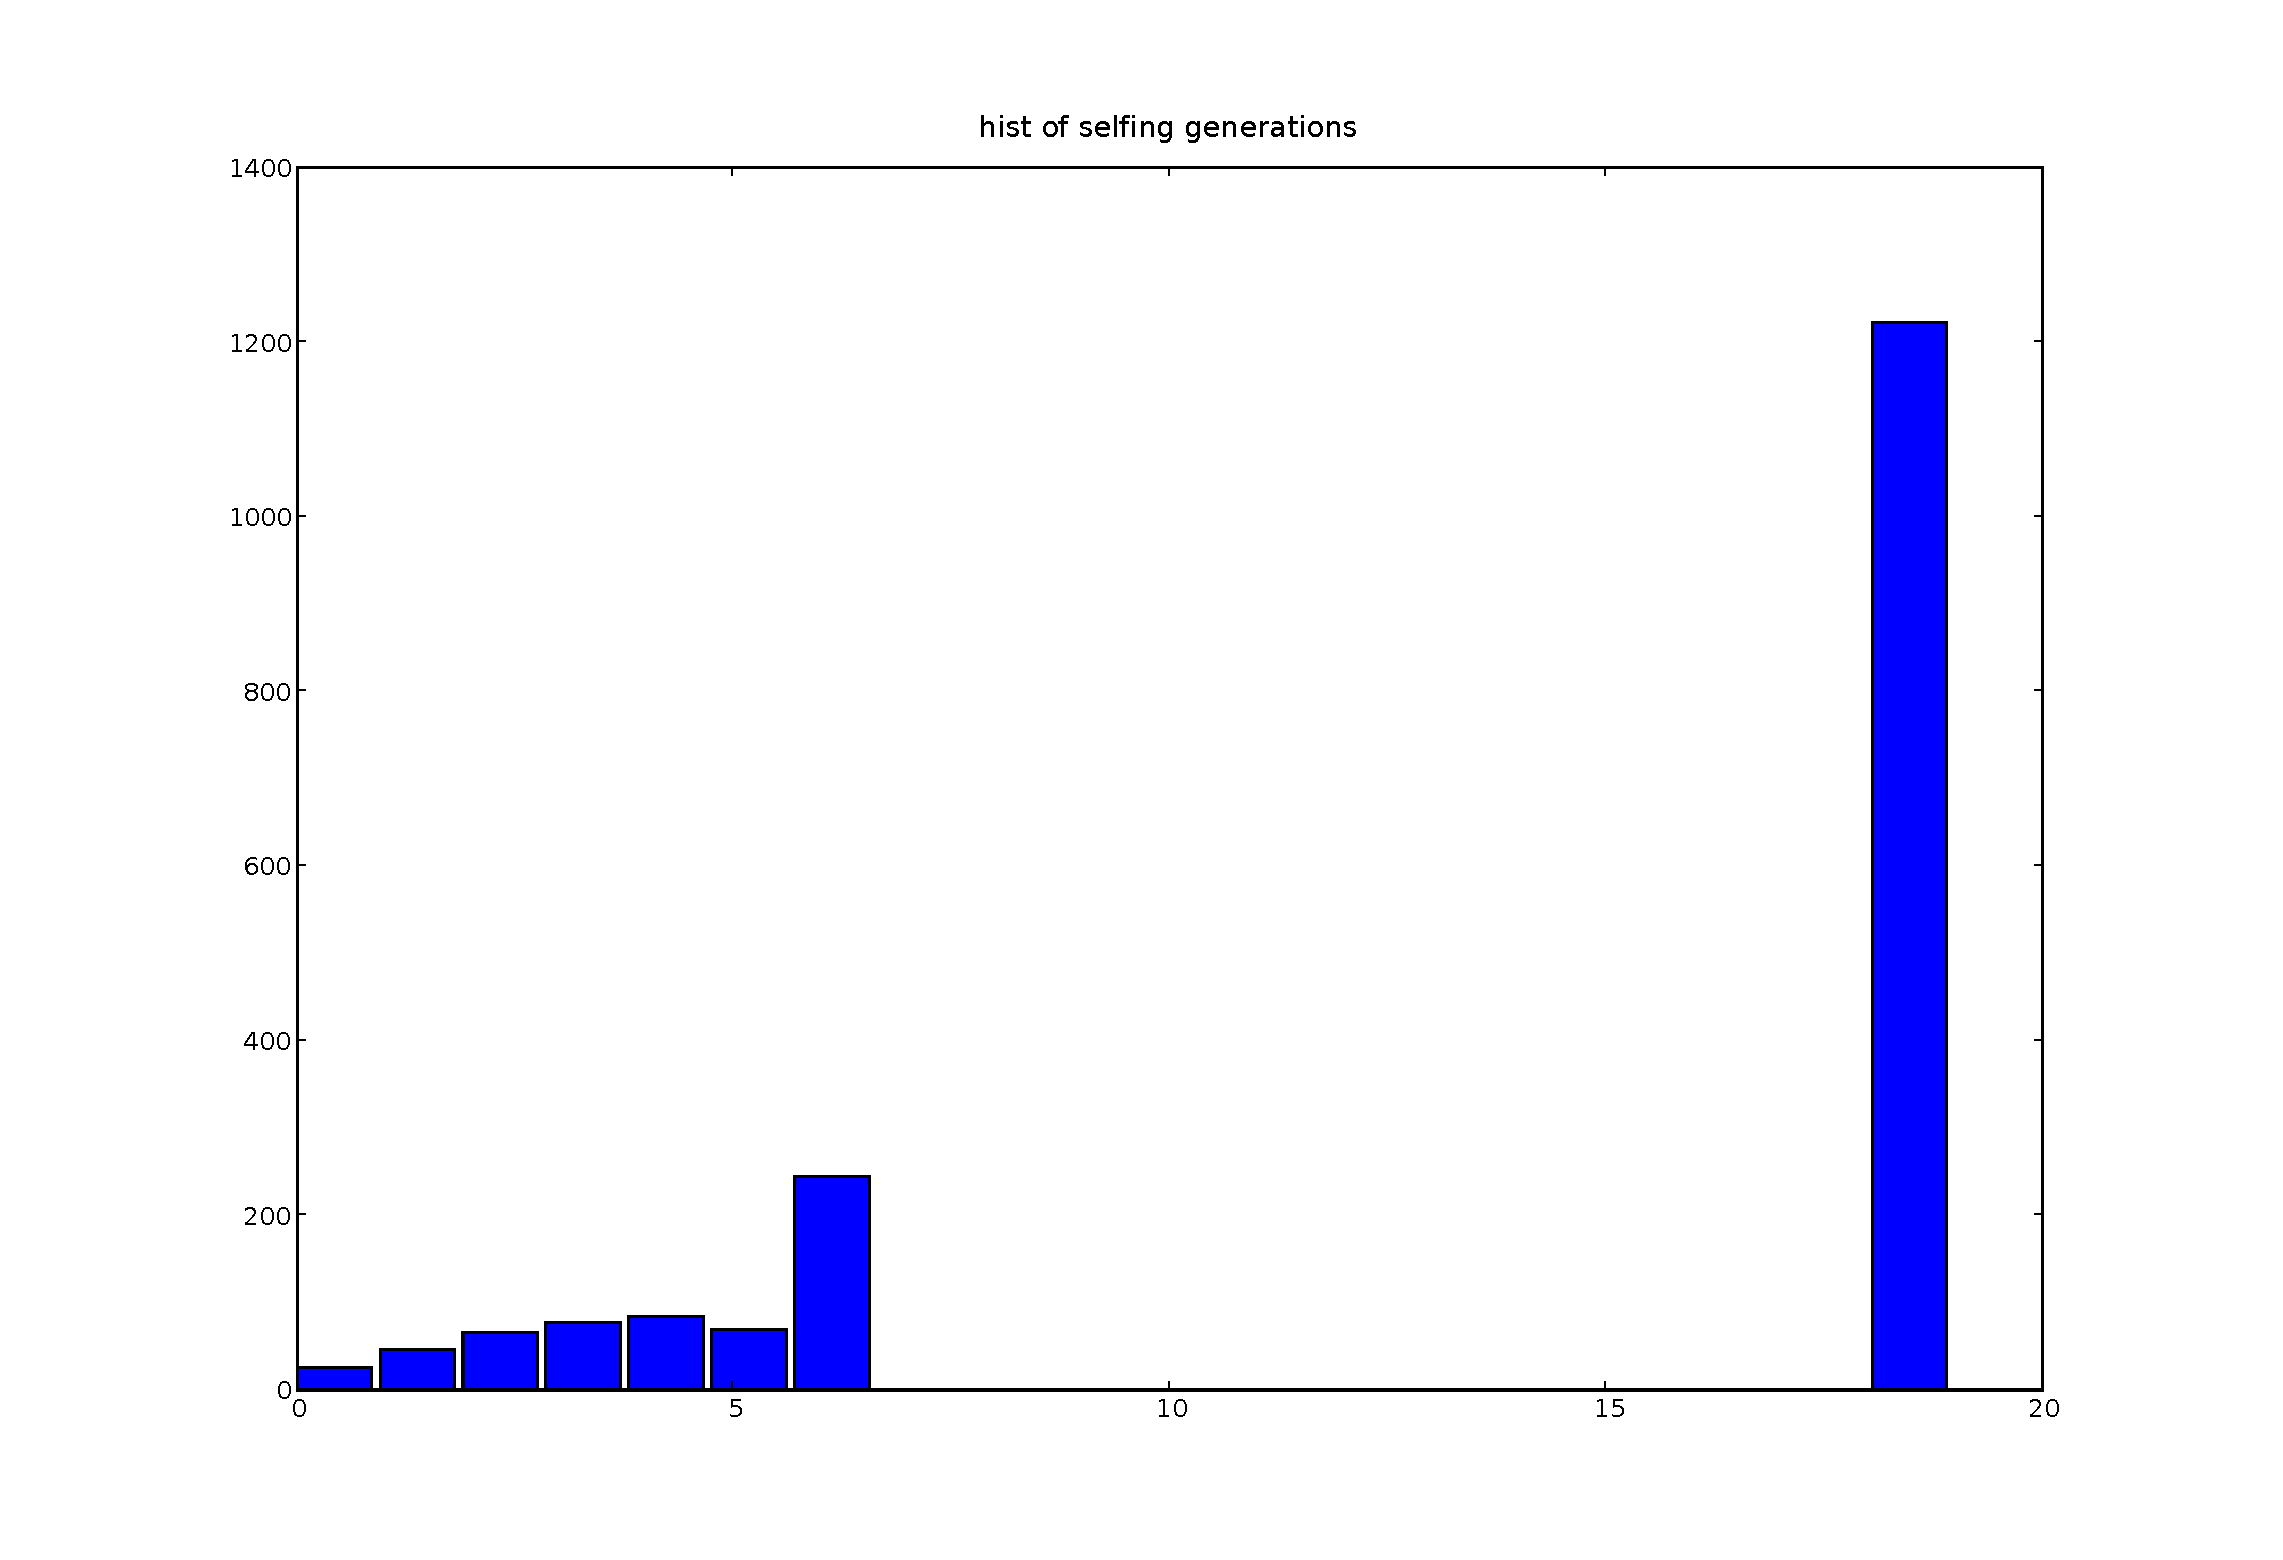
\includegraphics[width=1\textwidth]{figures/justin_data_y_b_filtered_estimate_selfing_generation_hist.eps}
\caption{}\label{f8}
\end{figure}

Figure~\ref{f9} is an example showing one strain with 0 selfing generations from the last outcrossing event.

\begin{figure}
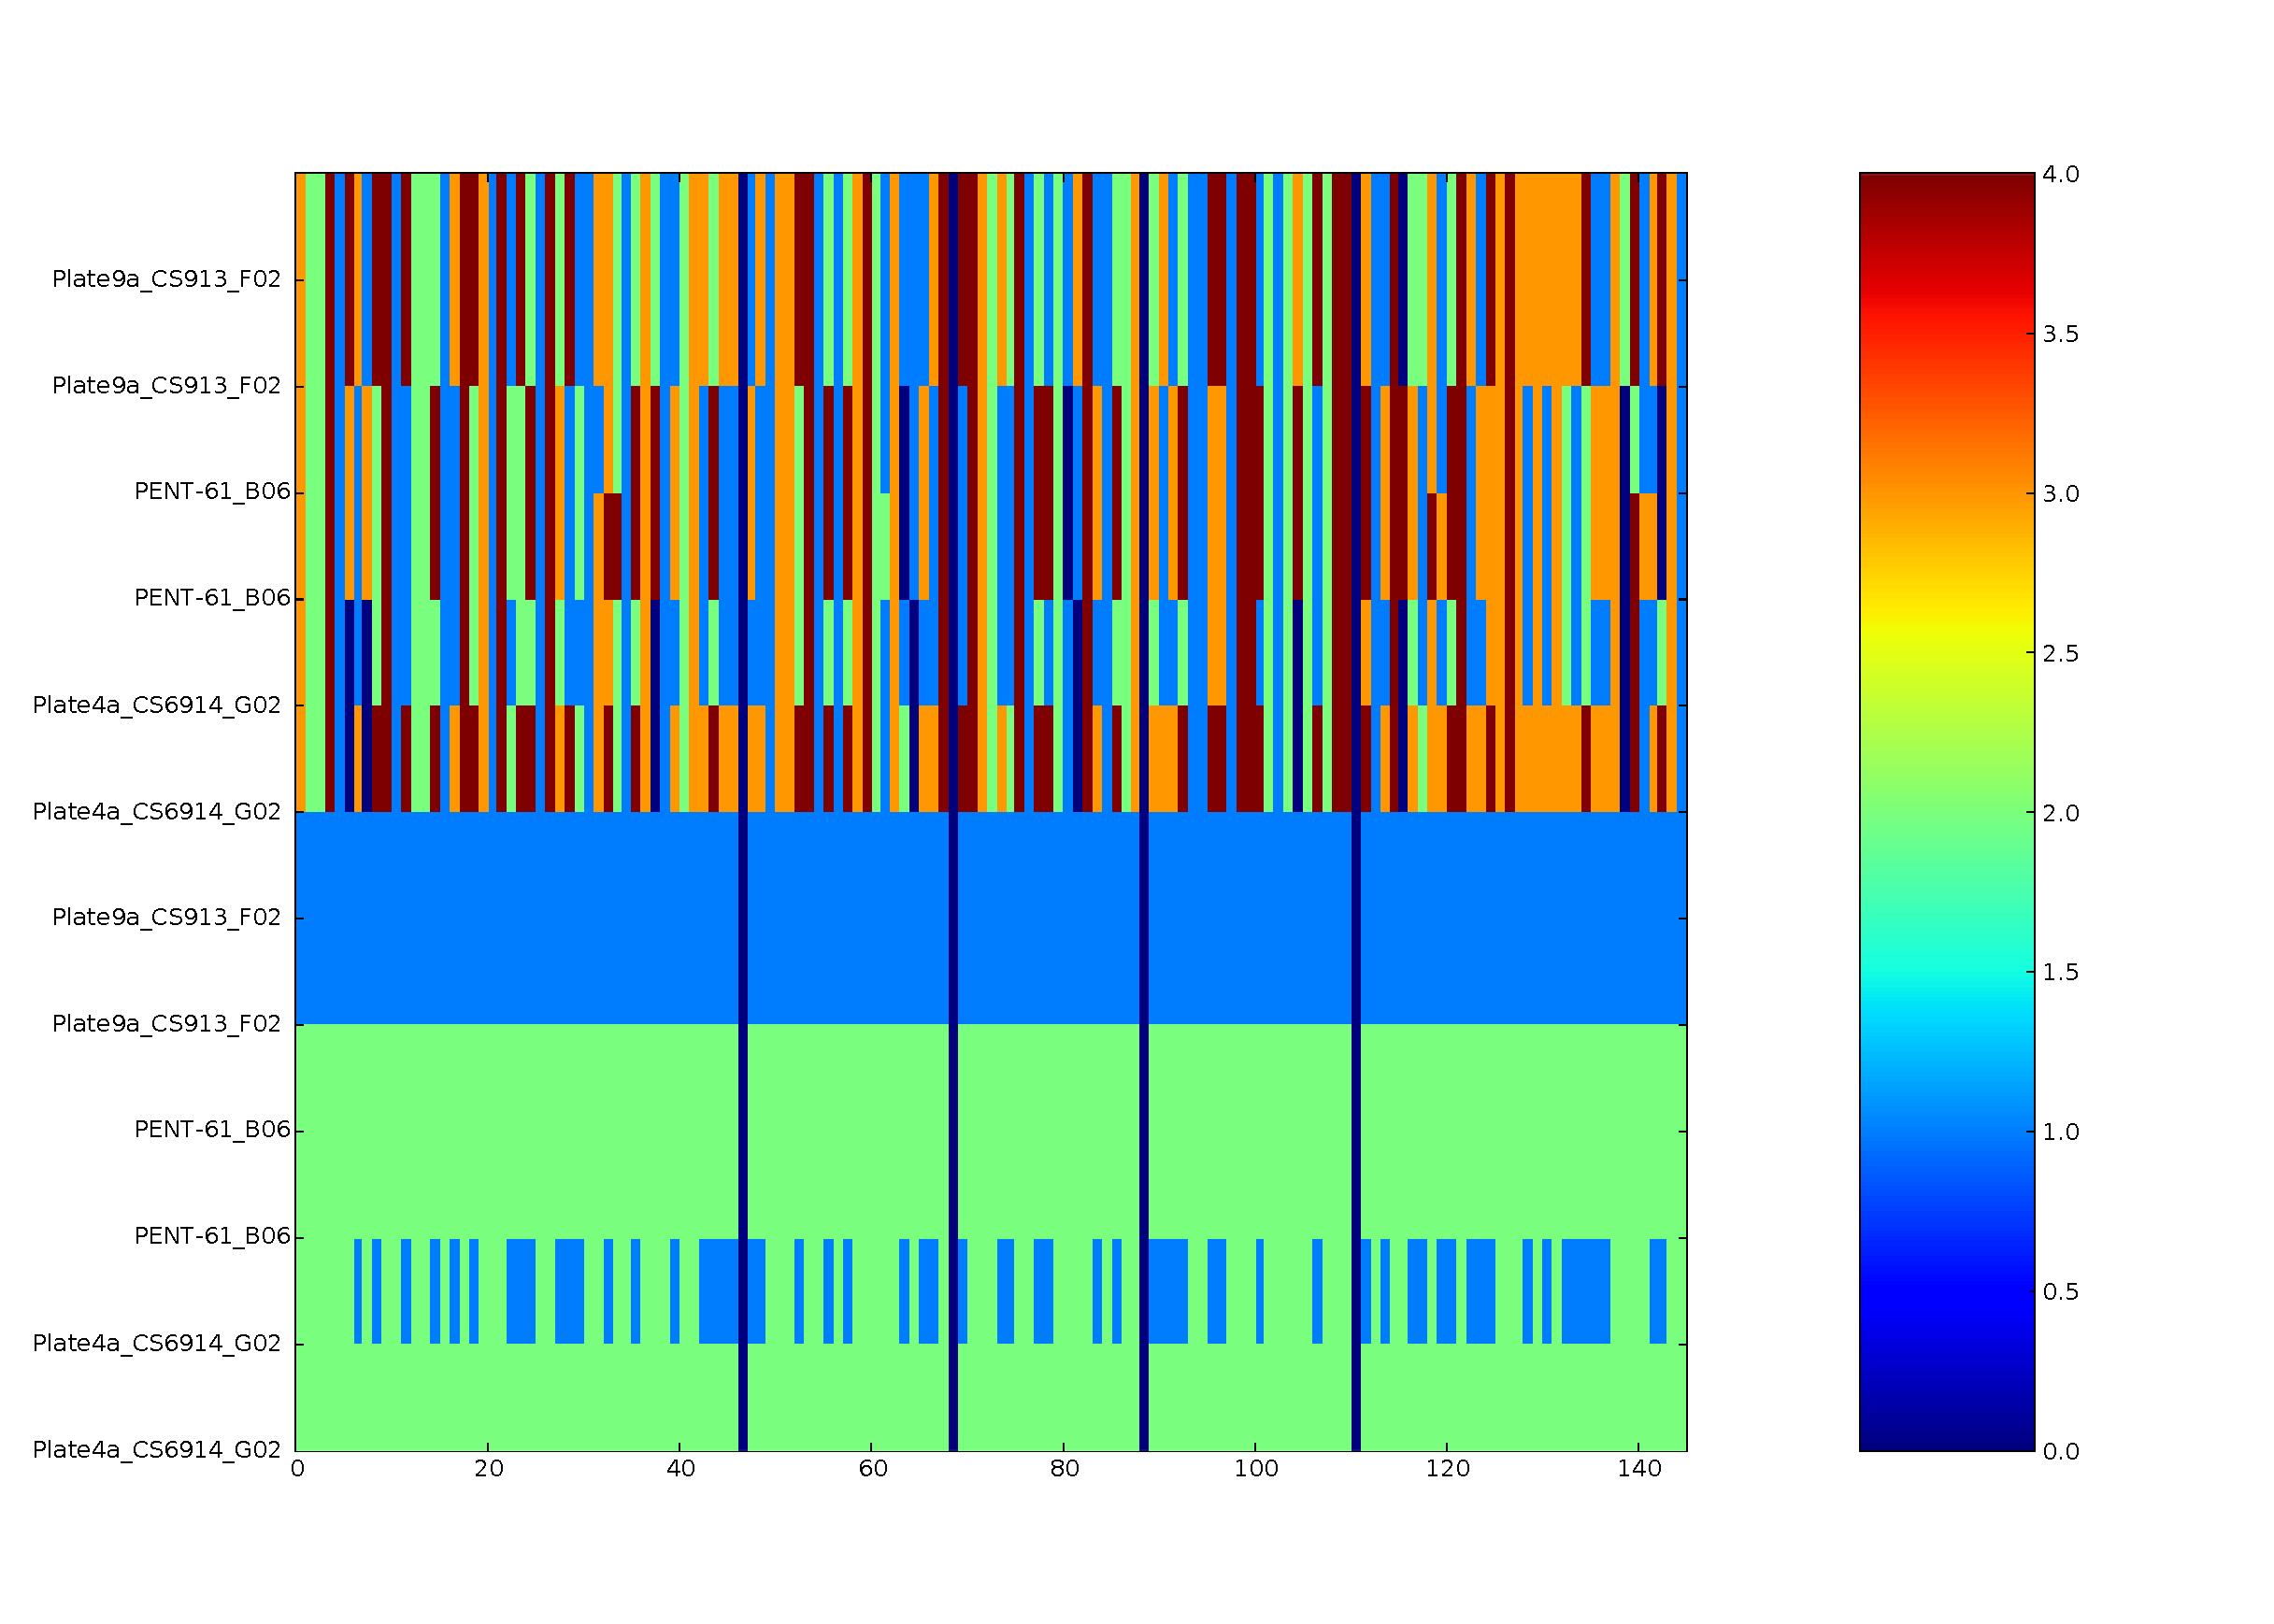
\includegraphics[width=1\textwidth]{figures/trio1.eps}
\caption{}\label{f9}
\end{figure}

\section{Estimate selfing rate}
Here gives a summary of the methods tried so far. the goal is to see whether there're major difference among different methods. the quick answer is no.

\subsection{Jarne2006~\cite{Jarne2006}}
simplest, single-locus, $F_{IS}$-based. $F_{IS} = 1-H_{obs}/H_e$, where $H_e$ is the expected heterozygosity, $H_e = 2pq$ and $H_{obs}$ is the observed heterozygosity. $s = 2F_{IS}/(1+F_{IS})$.

\subsection{Robertson1984~\cite{Robertson1984}}
single-locus, $F_{IS}$-based. not significantly different from Jarne2006. estimate is slightly higher than Jarne2006's. in several cases, it gives estimate slightly over 1.

\subsection{Weir1984~\cite{Weir1984}}
single-locus, multi-loci, $F_{IS},F_{ST}$-based. The single locus estimate gives similar result to Jarne2006 or Nordborg1997. But the multi-locus gives significantly lower estimate.

\subsection{Nordborg1997~\cite{Nordborg1997}}
single-locus, colascent-based. This estimate gives value equal to Weir1984's single-locus one.

\subsection{David2007~\cite{David2007}}
it's based on identity disequilibrium, which is an excess of heterozygotes or homozygotes across multiple loci. this method is most computing intensive and shows greatest difference.

\subsection{todo}
\begin{enumerate}
 \item Enjalbert2000~\cite{Enjalbert2000} method
 \item Simulate data with different selfing rate and apply different algorithms to see how effective different methods are.
\end{enumerate}

How to define a population remains a question. Gao2007~\cite{Gao2007}, Pritchard2000~\cite{Pritchard2000}, Guillot2005~\cite{Guillot2005} and Francois2006~\cite{Francois2006} have interesting solutions. But before figuring out how to define populations, we just tried a simple method.

\subsection{Selfing rates across globe}
Each population is formed via connecting close sites. There's a distance (great circle distance) threshold to determine how close sites within a population should be. For each population, its data undergoes a few preprocessing procedures. 1. remove strains with $>=40\%$ NA. 2. remove snps with $>=40\%$ NA. 3. remove snps with too many heterozygous inconsistent with the strains' homozygous state (detailed in a previous section).

so far 5km (120 populations), 10km (96 populations), 25km (66 populations) have been tried. The figures below are shown in this order for each particular region (England, Europe Continent, North America, Sweden).

In figures below, selfing rates are estimated by Jarne2006. Other methods (except David2007's) show minor differences most of the time. we'll come to the differing parts later. Each population is labeled by selfing rate X 1000. 0 denotes not enough data to make inference (at least 5 samples/strains). The diameter of the circle corresponds to the size of the population.

\subsubsection{Standard deviation of these selfing rates}

Due to the fact that Jarne2006's estimate is single-locus based, the selfing rate that's put on the map is the average of all loci. For those low average selfing rates, the std (standard deviation) is also bigger, which means for most loci of that population, selfing rate estimate is pretty close to 1 and just a few with a lot of heterozygous calls which pulls down the average. However remember, bad snps with too many heterozygous inconsistent with the strains' homozygous state have already been eliminated. These ones are probably not technical errors.

\subsubsection{Negative selfing rate estimates}
In short, negative estimates are caused by the excess of heterozygosity compared to the Hardy Weinberg prediction ($2pq$). Supposedly, inbreeding would cause a deficiency of heterozygosity. Possibly due to sampling and extremely minor allele frequency, excess is observed. The identity-disequilibrium-based David2007's method doesn't suffer this problem.

It's hard to see those selfing rates without significantly magnification. I have high-resolution eps figures.

\begin{figure}
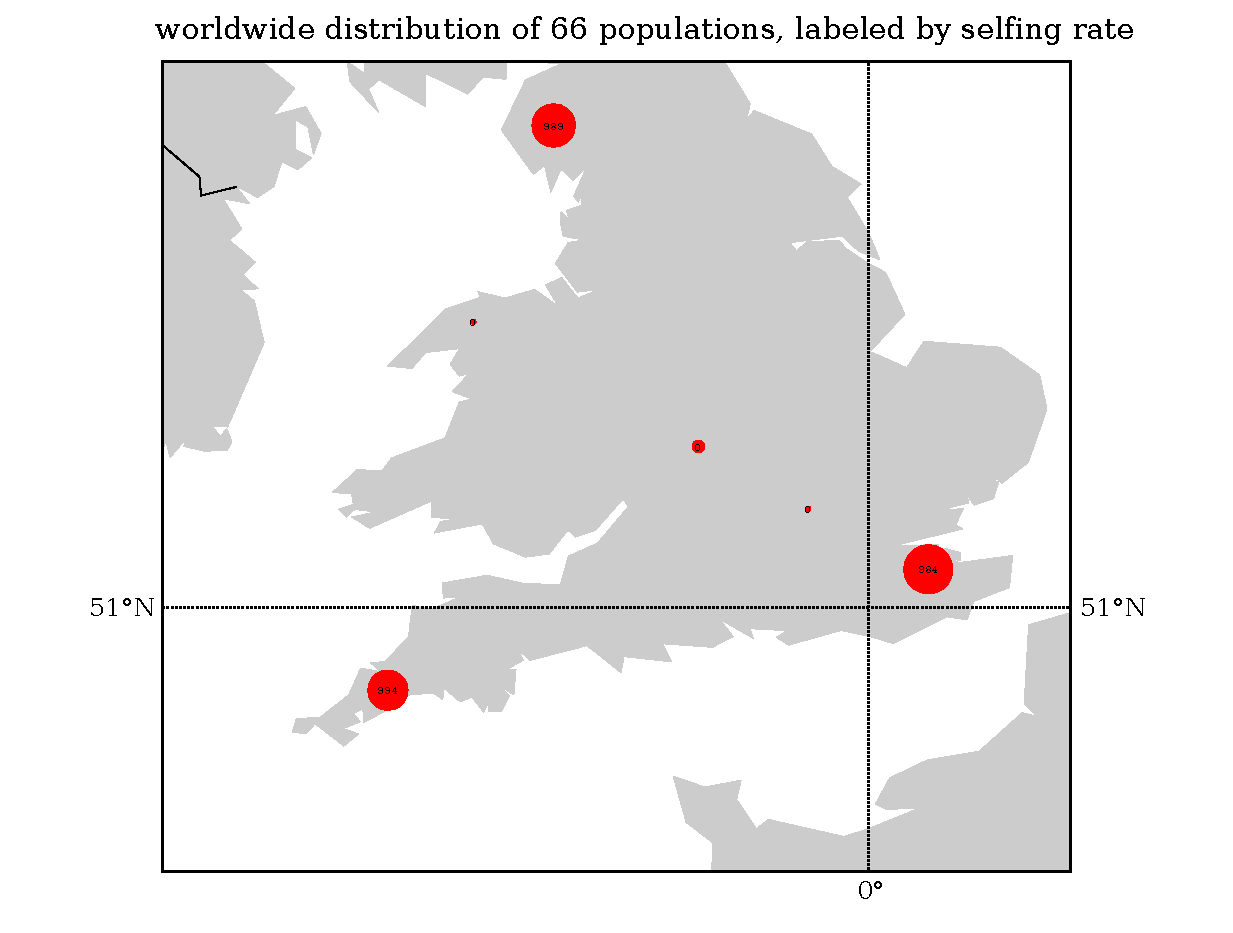
\includegraphics[width=1\textwidth]{figures/s0829popid2ecotypeid_25_Eng__7_49_2_55_l3y1_pop_map.eps}
\caption{England}\label{f12}
\end{figure}

\begin{figure}
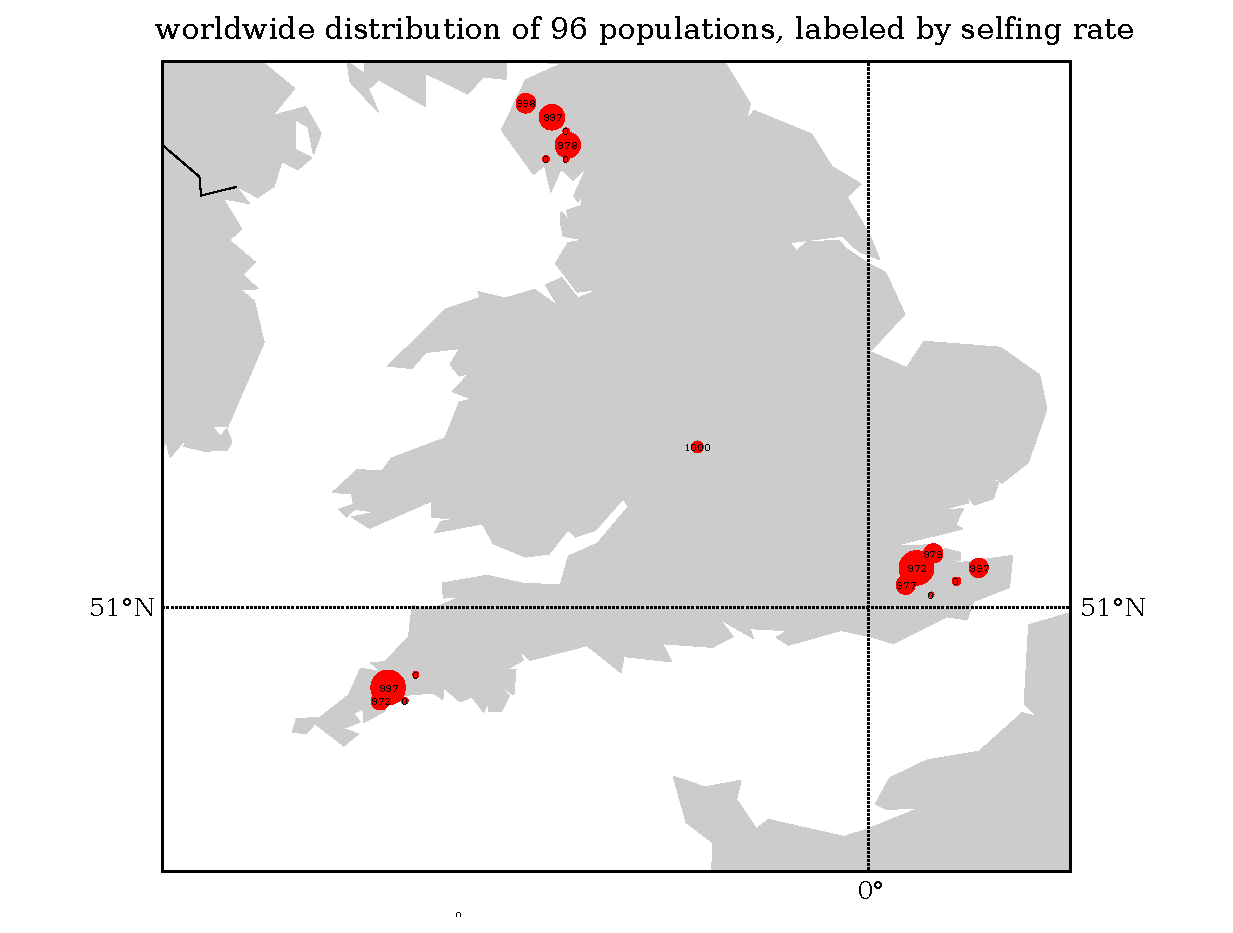
\includegraphics[width=1\textwidth]{figures/s0829popid2ecotypeid_10_Eng__7_49_2_55_l3y1_pop_map.eps}
\caption{England}\label{f11}
\end{figure}

\begin{figure}
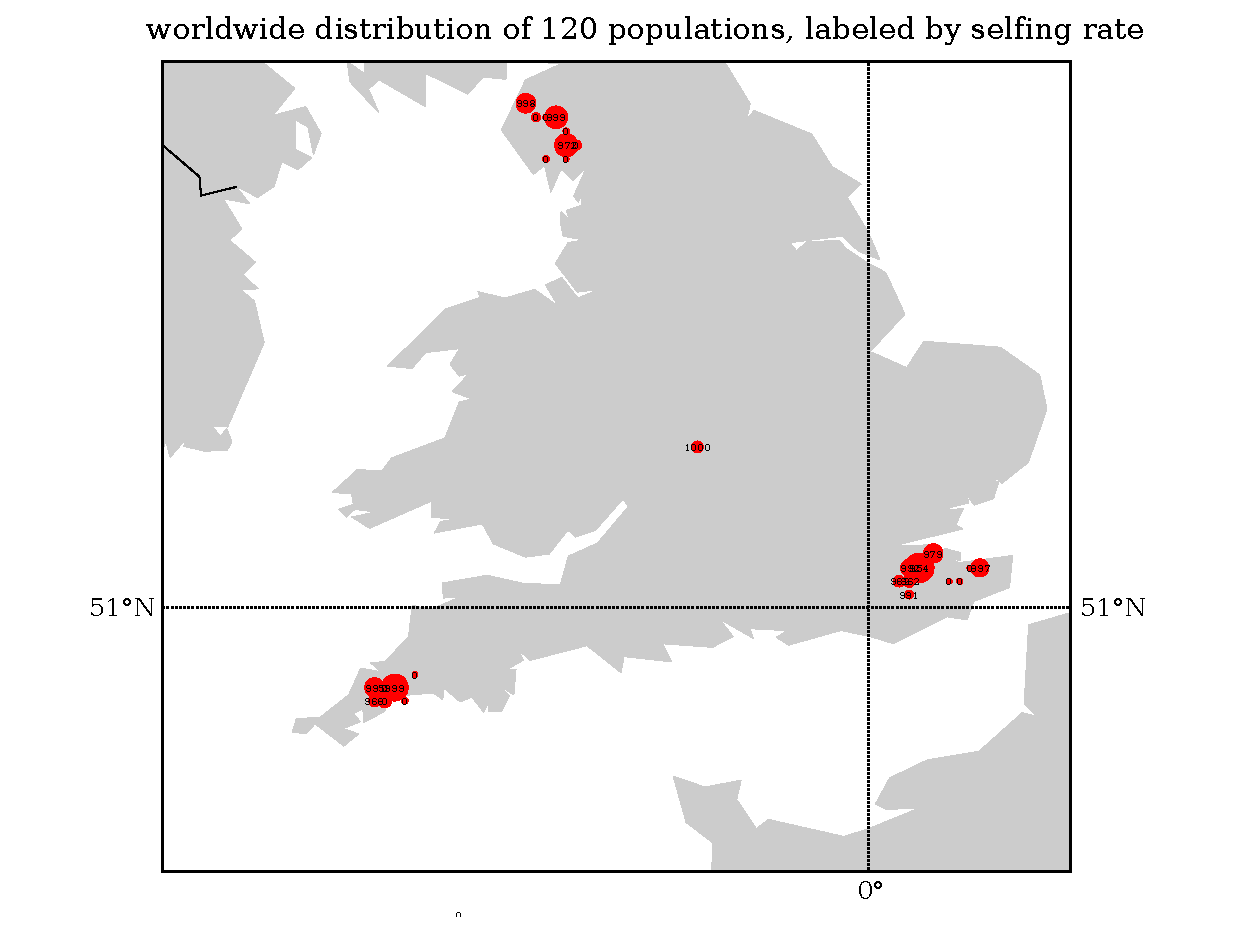
\includegraphics[width=1\textwidth]{figures/s0829popid2ecotypeid_5_Eng__7_49_2_55_l3y1_pop_map.eps}
\caption{England}\label{f23}
\end{figure}


\begin{figure}
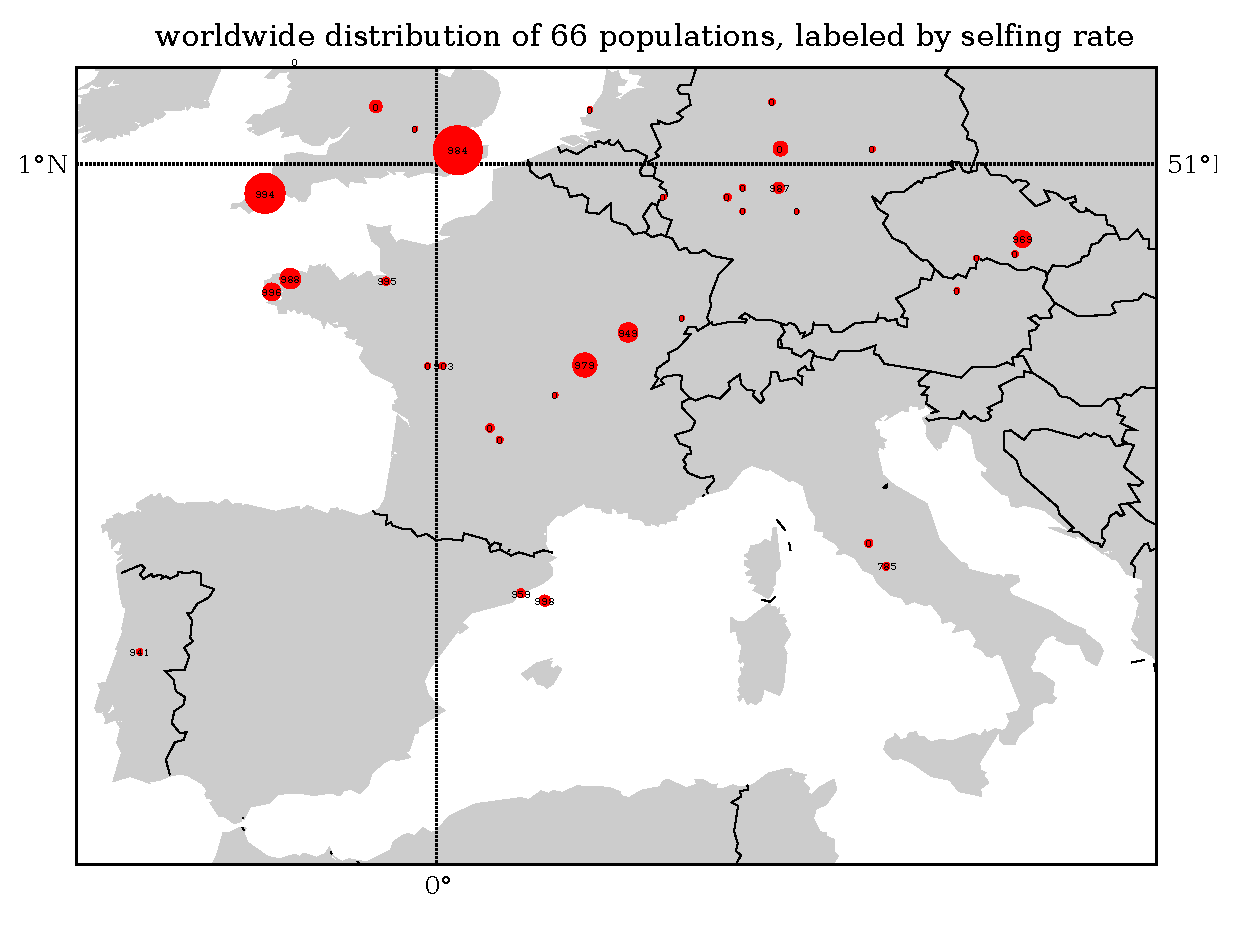
\includegraphics[width=1\textwidth]{figures/s0829popid2ecotypeid_25_EurCont__10_35_20_53_l3y1_pop_map.eps}
\caption{Europe Continent}\label{f15}
\end{figure}

\begin{figure}
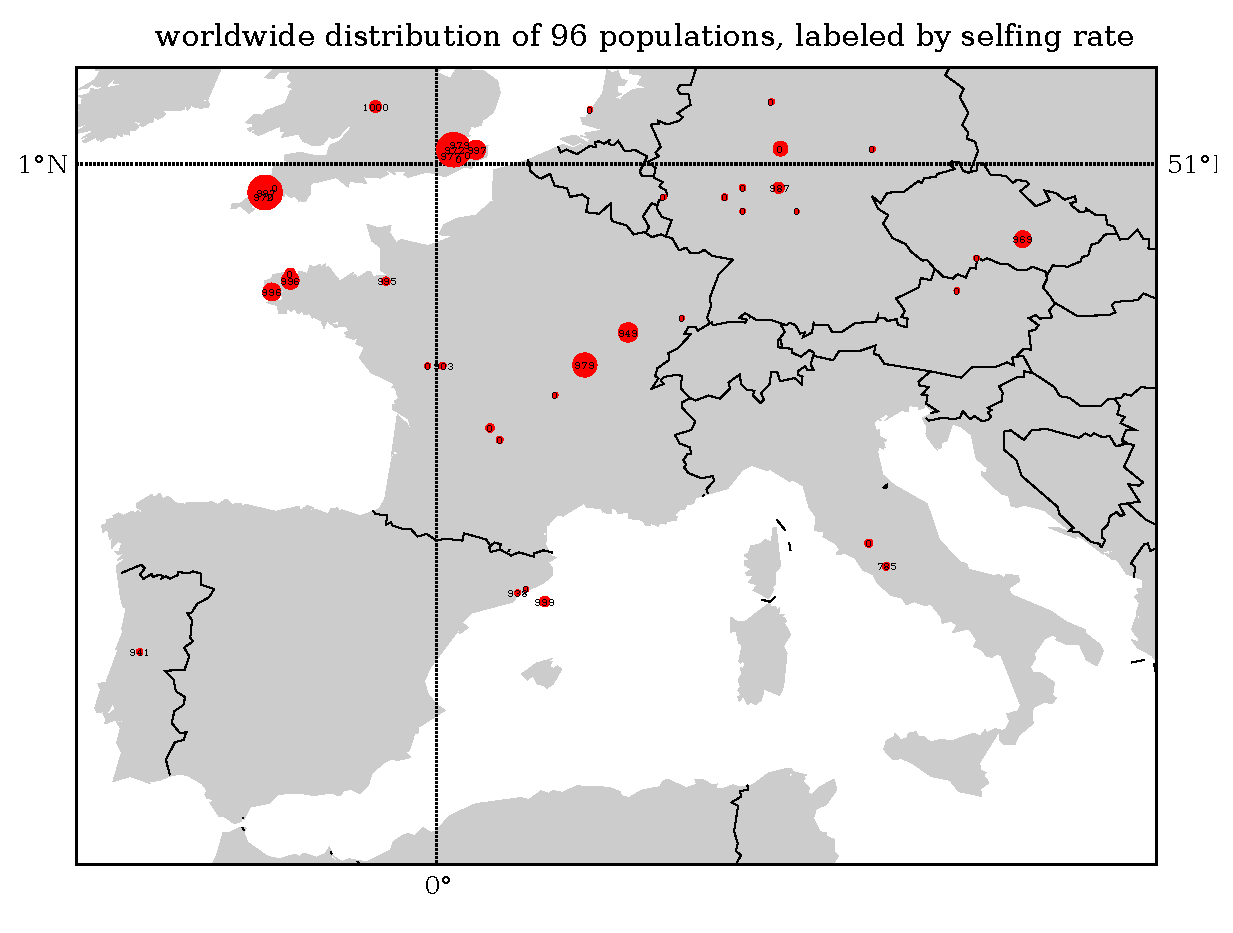
\includegraphics[width=1\textwidth]{figures/s0829popid2ecotypeid_10_EurCont__10_35_20_53_l3y1_pop_map.eps}
\caption{Europe Continent}\label{f14}
\end{figure}

\begin{figure}
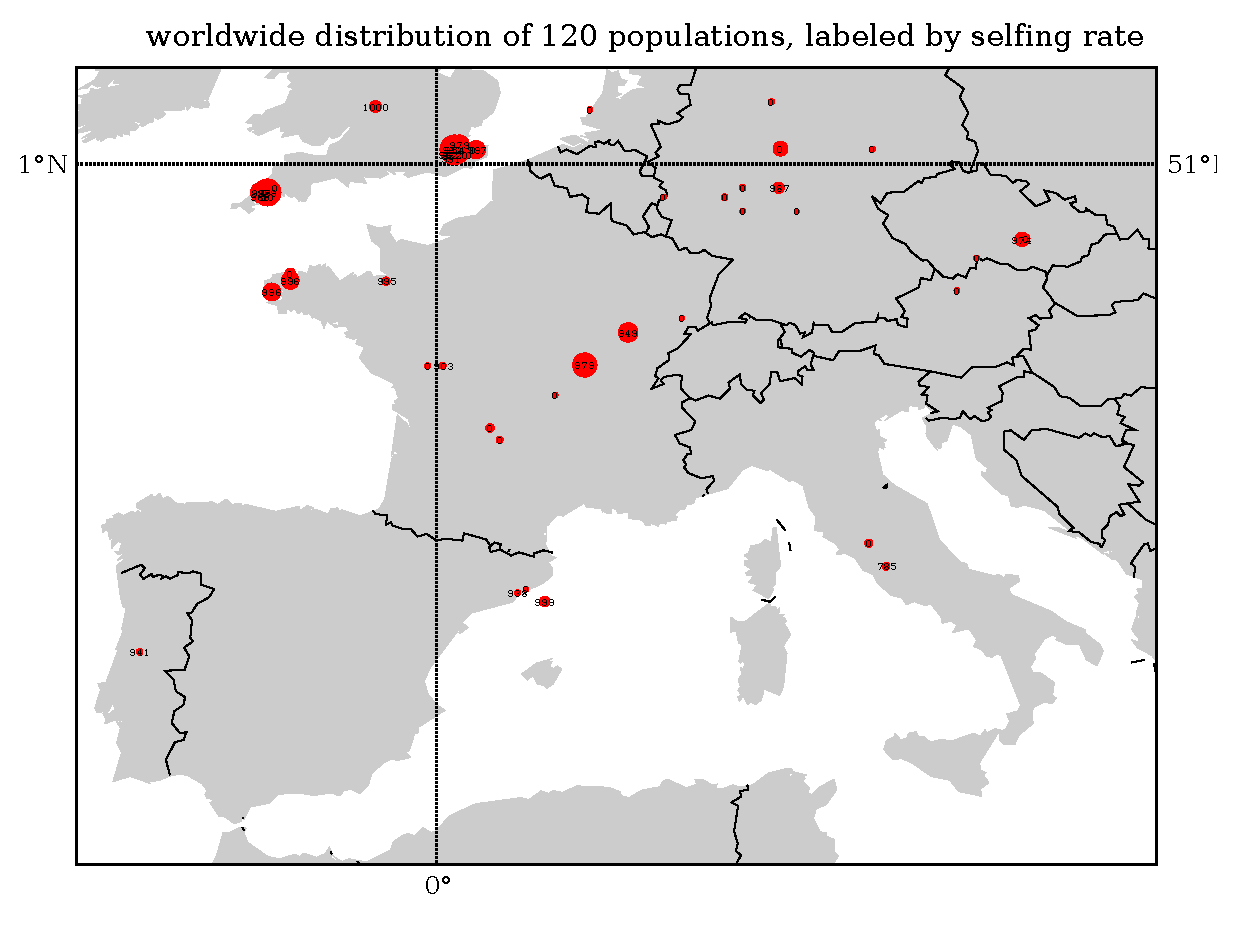
\includegraphics[width=1\textwidth]{figures/s0829popid2ecotypeid_5_EurCont__10_35_20_53_l3y1_pop_map.eps}
\caption{Europe Continent}\label{f13}
\end{figure}



\begin{figure}
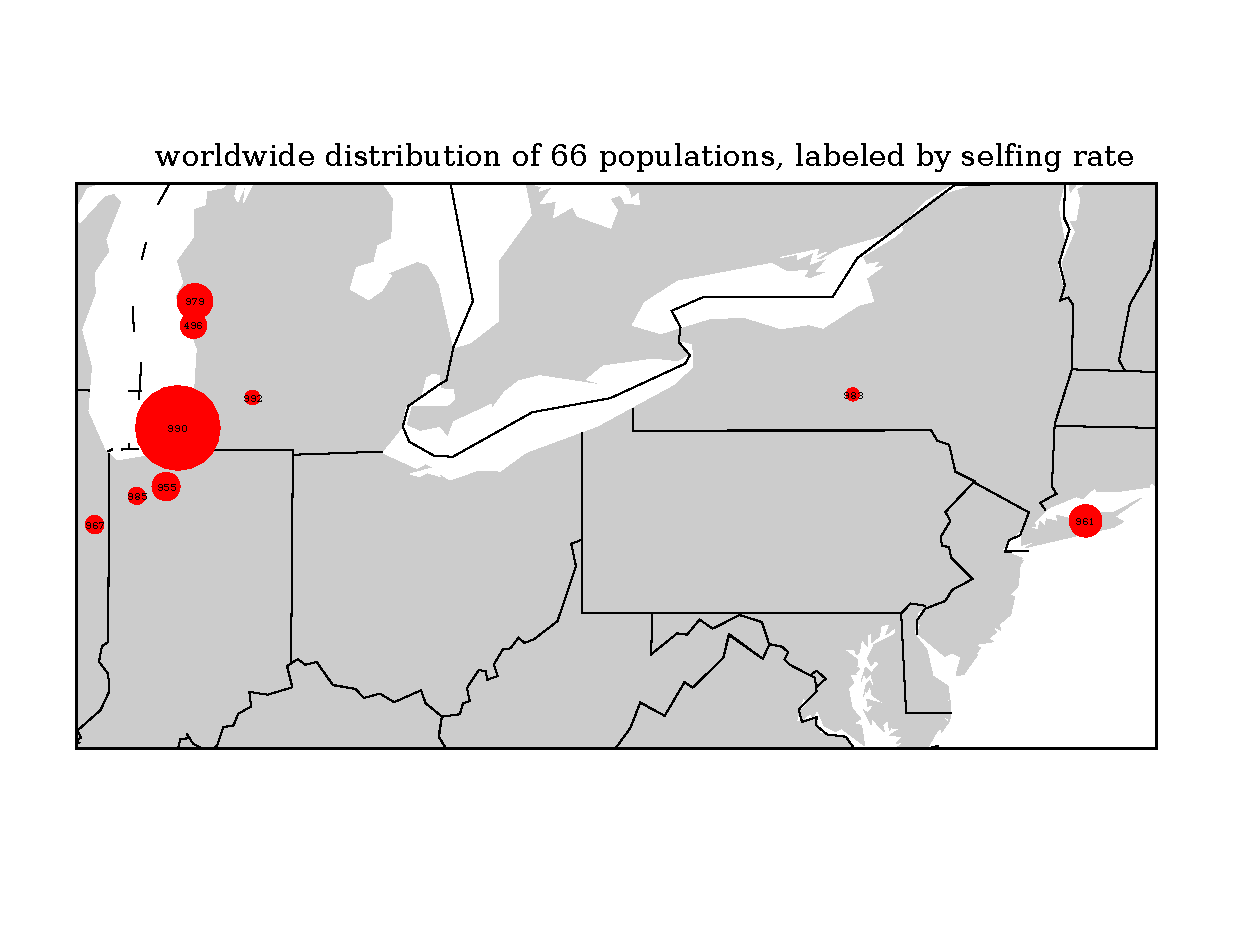
\includegraphics[width=1\textwidth]{figures/s0829popid2ecotypeid_25_NorAm__88_38__72_45_l3y1_pop_map.eps}
\caption{North America}\label{f18}
\end{figure}

\begin{figure}
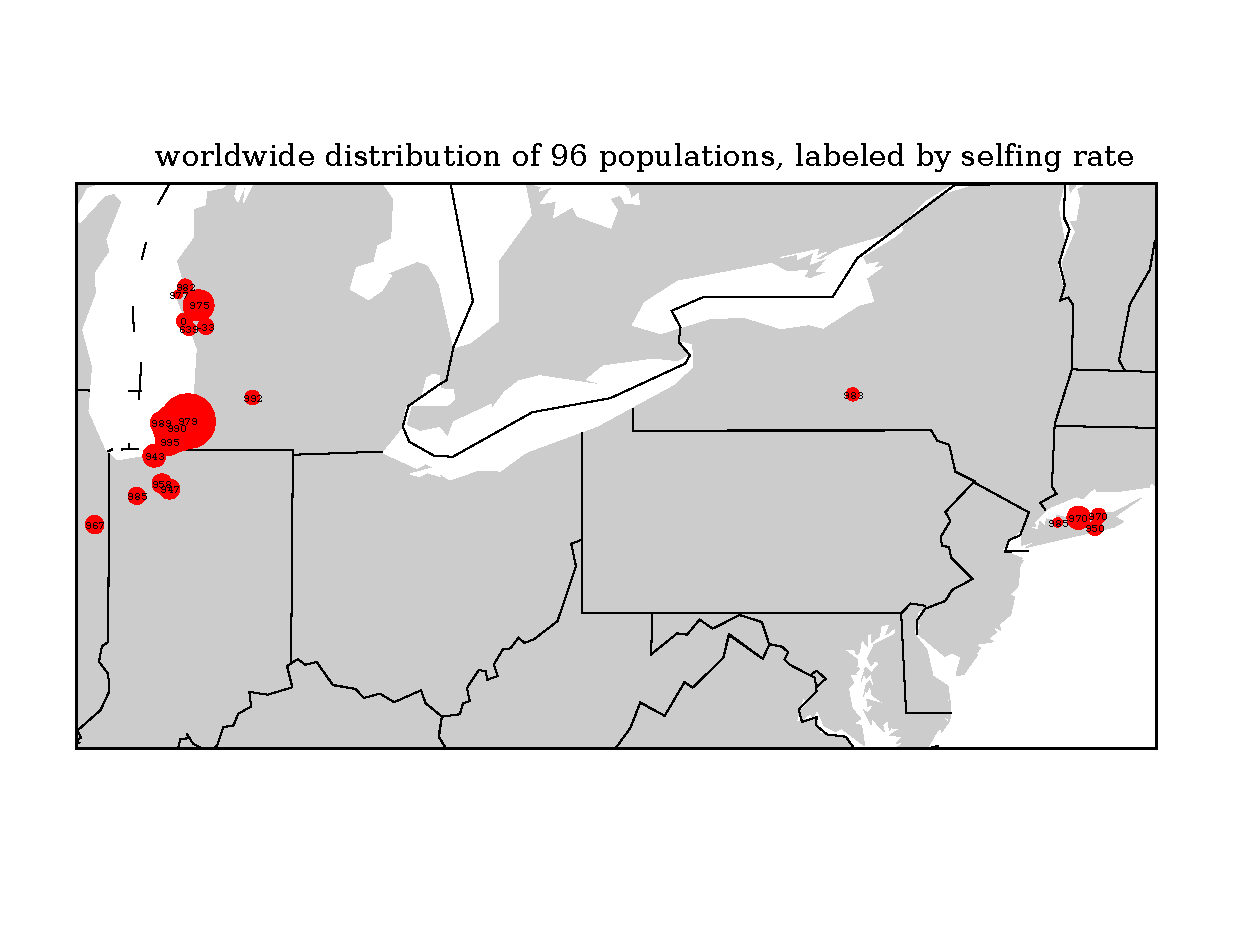
\includegraphics[width=1\textwidth]{figures/s0829popid2ecotypeid_10_NorAm__88_38__72_45_l3y1_pop_map.eps}
\caption{North America}\label{f17}
\end{figure}

\begin{figure}
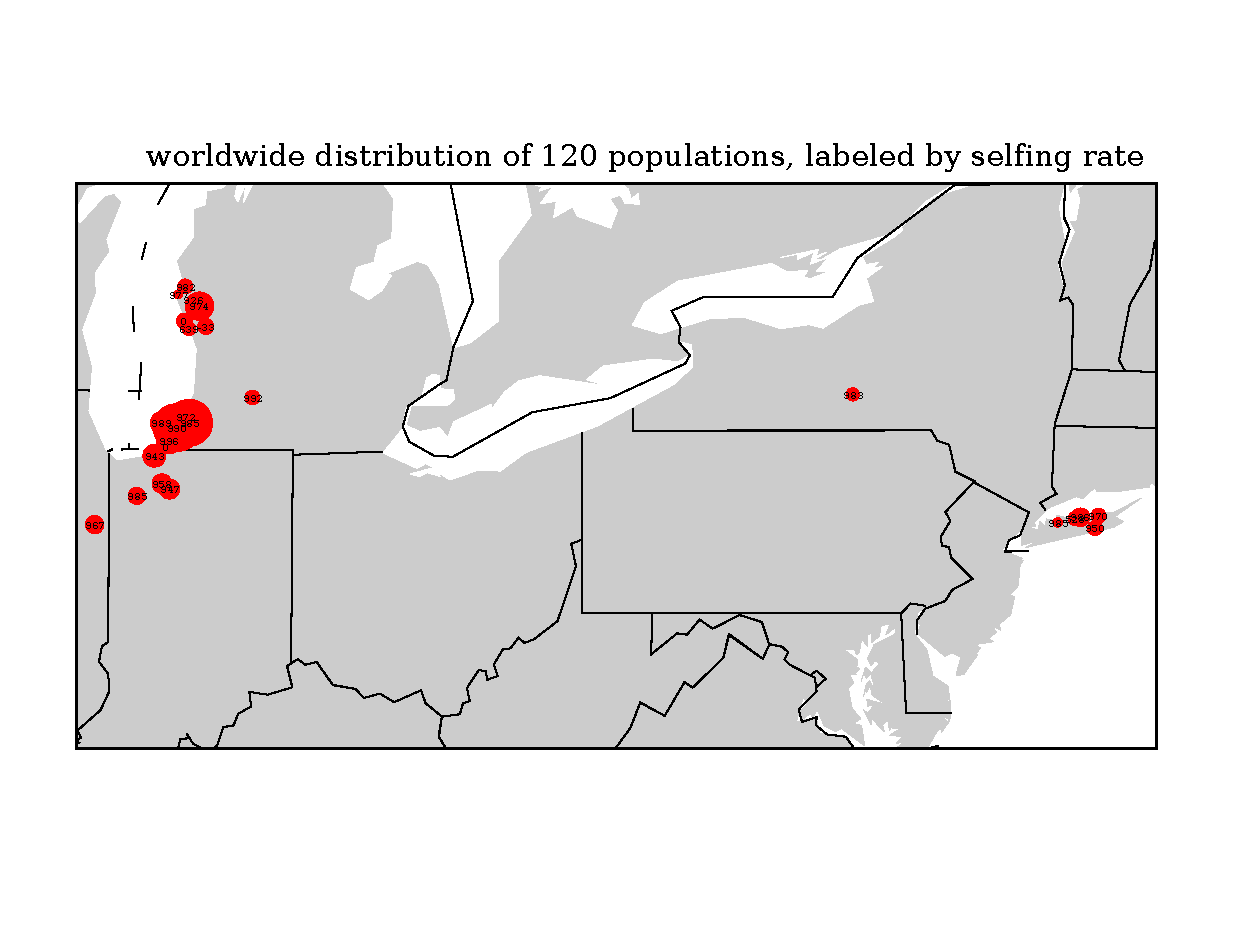
\includegraphics[width=1\textwidth]{figures/s0829popid2ecotypeid_5_NorAm__88_38__72_45_l3y1_pop_map.eps}
\caption{North America}\label{f16}
\end{figure}


\begin{figure}
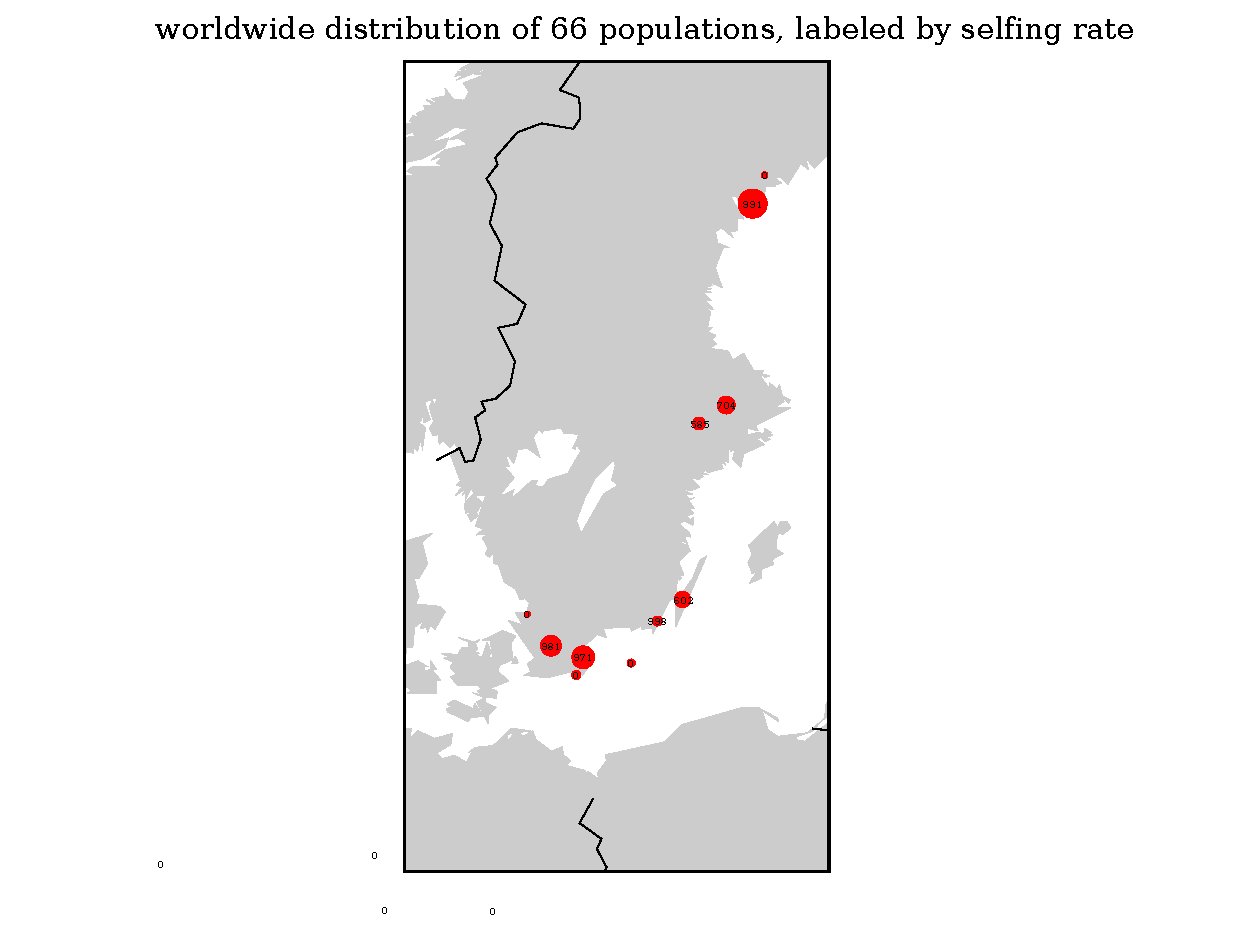
\includegraphics[width=1\textwidth]{figures/s0829popid2ecotypeid_25_Swe_10_52_20_65_l3y1_pop_map.eps}
\caption{Sweden}\label{f21}
\end{figure}

\begin{figure}
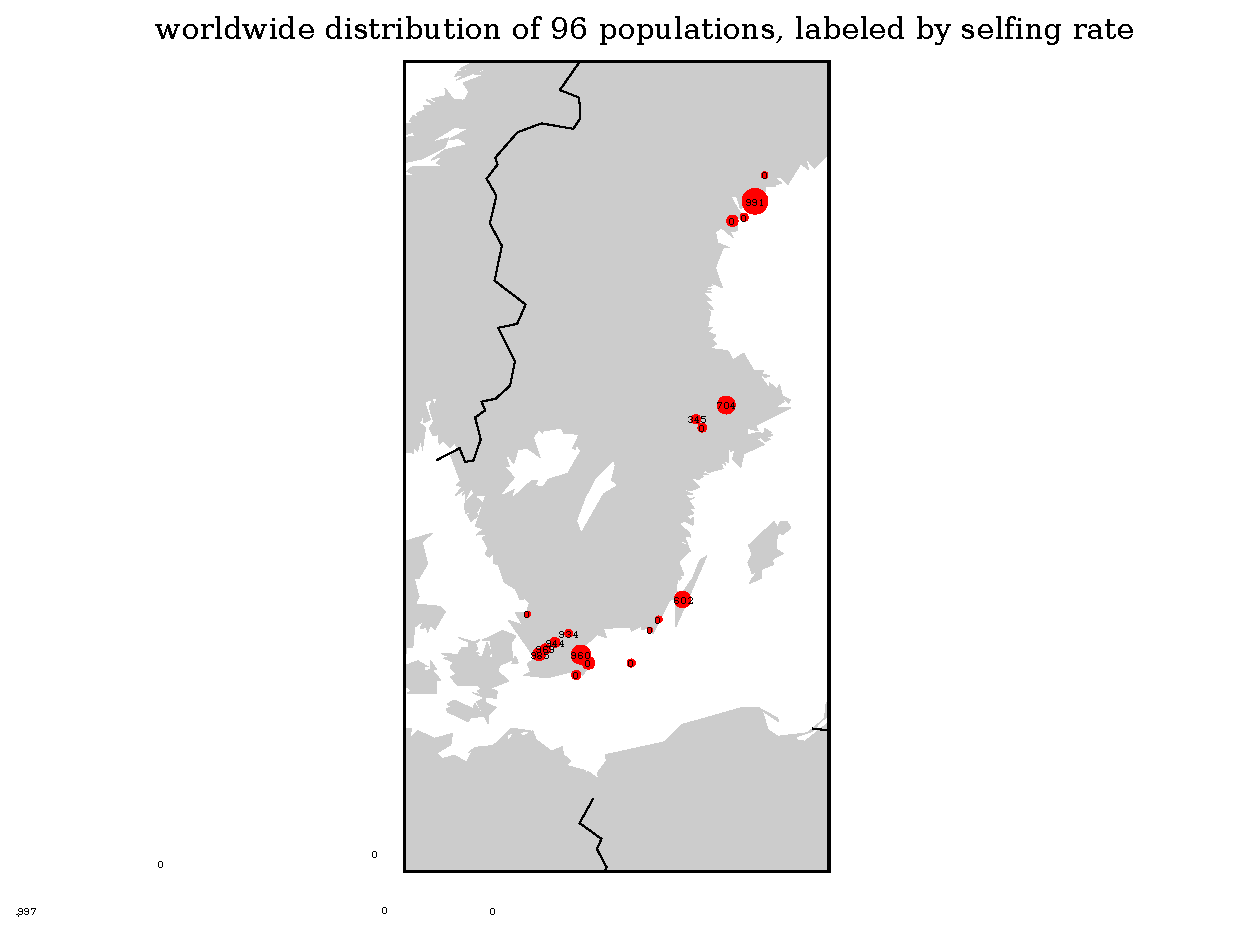
\includegraphics[width=1\textwidth]{figures/s0829popid2ecotypeid_10_Swe_10_52_20_65_l3y1_pop_map.eps}
\caption{Sweden}\label{f20}
\end{figure}

\begin{figure}
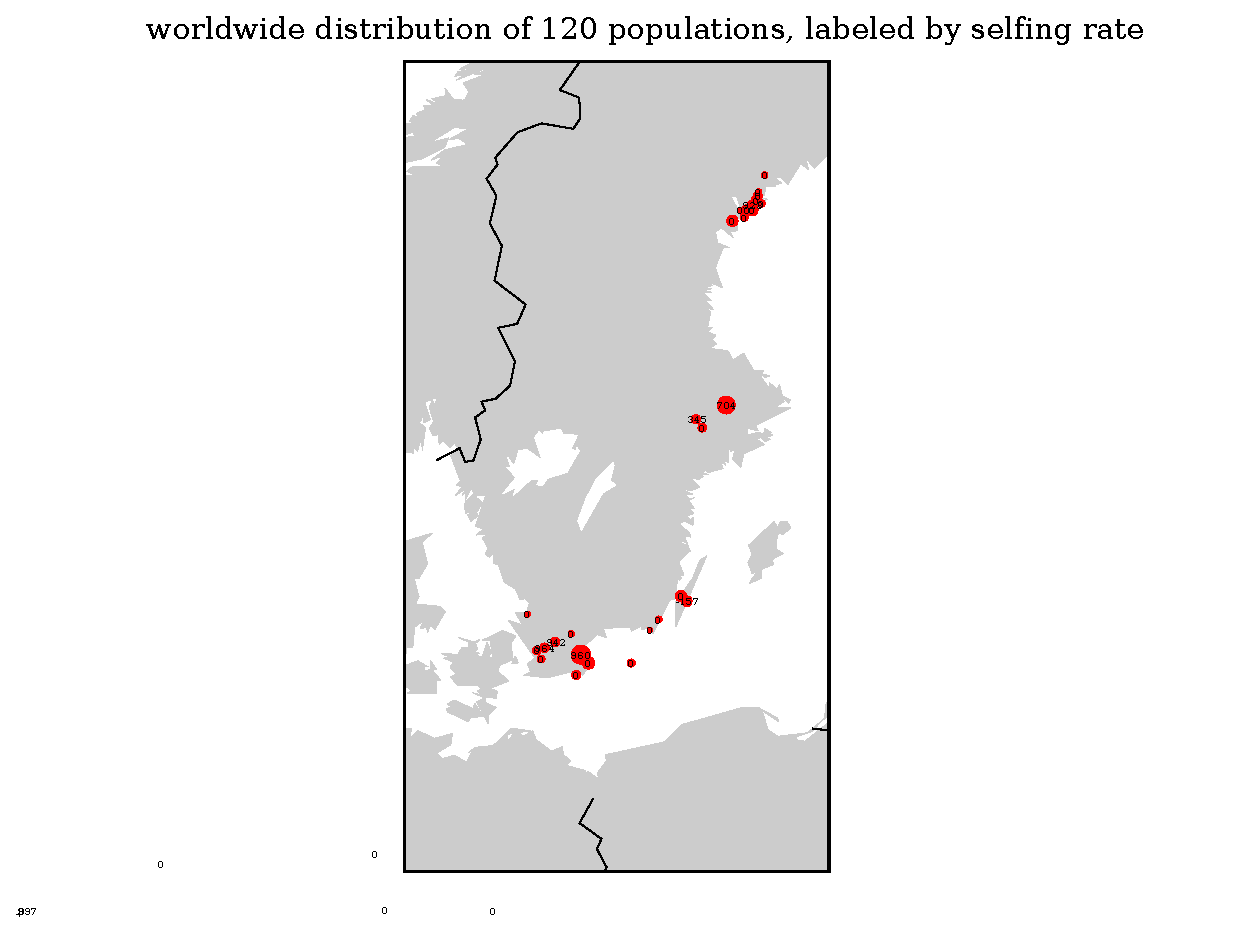
\includegraphics[width=1\textwidth]{figures/s0829popid2ecotypeid_5_Swe_10_52_20_65_l3y1_pop_map.eps}
\caption{Sweden}\label{f19}
\end{figure}


\bibliography{outcrossing}
\bibliographystyle{plain}

\end{document}
